% Copyright 2007, 2008, 2009 Elsevier Ltd
%
% This file is part of the 'Elsarticle Bundle'.
% ---------------------------------------------
%
% It may be distributed under the conditions of the LaTeX Project Public
% License, either version 1.2 of this license or (at your option) any
% later version.  The latest version of this license is in
%    http://www.latex-project.org/lppl.txt
% and version 1.2 or later is part of all distributions of LaTeX
% version 1999/12/01 or later c.
%
% The list of all files belonging to the 'Elsarticle Bundle' is
% given in the file `manifest.txt'.
%

% Template article for Elsevier's document class `elsarticle'
% with harvard style bibliographic references
% SP 2008/03/01
%
%
%
% $Id: elsarticle-template-harv.tex 4 2009-10-24 08:22:58Z rishi $
%
%
\documentclass[preprint,authoryear,12pt]{elsarticle}

% Use the option review to obtain double line spacing
%\documentclass[authoryear,preprint,review,12pt]{elsarticle}

% Use the options 1p,twocolumn; 3p; 3p,twocolumn; 5p; or 5p,twocolumn
% for a journal layout:
%\documentclass[final,authoryear,1p,times]{elsarticle}
%\documentclass[final,authoryear,1p,times,twocolumn]{elsarticle}
%\documentclass[final,authoryear,3p,times]{elsarticle}
%\documentclass[final,authoryear,3p,times,twocolumn]{elsarticle}
%\documentclass[final,authoryear,5p,times]{elsarticle}
%\documentclass[final,authoryear,5p,times,twocolumn]{elsarticle}

%% if you use PostScript figures in your article
%% use the graphics package for simple commands
%% \usepackage{graphics}
%\usepackage{cases}
%% or use the graphicx package for more complicated commands
\usepackage{graphicx}
%% or use the epsfig package if you prefer to use the old commands
\usepackage{epsfig}

\usepackage{comment}

\usepackage{epstopdf}
\usepackage{pdflscape}
\usepackage{bm}
\usepackage{hyperref,url}
\hypersetup{colorlinks=true, urlcolor=blue, linkcolor=blue, citecolor=red}

%% The amssymb package provides various useful mathematical symbols
\usepackage{amssymb,amsmath,array}
%The amsthm package provides extended theorem environments
\usepackage{amsthm}
\usepackage{graphicx}
\usepackage{subfigure}  
%% The lineno packages adds line numbers. Start line numbering with
%% \begin{linenumbers}, end it with \end{linenumbers}. Or switch it on
%% for the whole article with \linenumbers after \end{frontmatter}.
%% \usepackage{lineno}

\usepackage{lscape}

%% natbib.sty is loaded by default. However, natbib options can be
%% provided with \biboptions{...} command. Following options are
%% valid:

%%   round  -  round parentheses are used (default)
%%   square -  square brackets are used   [option]
%%   curly  -  curly braces are used      {option}
%%   angle  -  angle brackets are used    <option>
%%   semicolon  -  multiple citations separated by semi-colon (default)
%%   colon  - same as semicolon, an earlier confusion
%%   comma  -  separated by comma
%%   authoryear - selects author-year citations (default)
%%   numbers-  selects numerical citations
%%   super  -  numerical citations as superscripts
%%   sort   -  sorts multiple citations according to order in ref. list
%%   sort&compress   -  like sort, but also compresses numerical citations
%%   compress - compresses without sorting
%%   longnamesfirst  -  makes first citation full author list
%%
%% \biboptions{longnamesfirst,comma}

% \biboptions{}

\newcommand{\JGnote}[1]{\fbox{\parbox{\textwidth}{ \color{blue} JG Note $\Rightarrow$ #1}}}
\newcommand{\red}{\textcolor{red}}
\journal{Advances in Water Resources}

\begin{document}

\begin{frontmatter}

%% Title, authors and addresses

%% use the tnoteref command within \title for footnotes;
%% use the tnotetext command for the associated footnote;
%% use the fnref command within \author or \address for footnotes;
%% use the fntext command for the associated footnote;
%% use the corref command within \author for corresponding author footnotes;
%% use the cortext command for the associated footnote;
%% use the ead command for the email address,
%% and the form \ead[url] for the home page:
%%
%% \title{Title\tnoteref{label1}}
%% \tnotetext[label1]{}
%% \author{Name\corref{cor1}\fnref{label2}}
%% \ead{email address}
%% \ead[url]{home page}
%% \fntext[label2]{}
%% \cortext[cor1]{}
%% \address{Address\fnref{label3}}
%% \fntext[label3]{}

\title{Numerical Investigation of Multi-Fluid Flows through Dual Saturated-Unsaturated Porous Media}

%% use optional labels to link authors explicitly to addresses:
\author[UoA]{K. Christou} \author[UoA,UFRGS]{W.C. Rad\"unz}  \author[UoA]{B. Lashore} 
\author[UoA]{J.L.M.A. Gomes\corref{cor1}}\ead{jefferson.gomes@abdn.ac.uk}

\cortext[cor1]{Corresponding author.}
\address[UoA]{Environmental and Industrial Fluid Mechanics Group, School of Engineering, University of Aberdeen, UK}
\address[UFRGS]{Engineering School, Federal University of Rio Grande do Sul, Brazil}

\begin{abstract} 
Numerical modelling of multiphase flow in porous media has a wide range of applications in science and engineering. Continuity equation and the Darcy's law govern the processes, while pressure, velocity, saturation and permeability are quantities that define the behaviour of the flow. A novel control finite element method (CVFEM) is used to discretize the governing equations that will solve the multi-fluid porous media flow model. The current model is the basis of a general purpose flow simulator that is equipped with anisotropic mesh adaptivity techniques to increase the computational accuracy of numerical methods used in geophysical fluid mechanics. The governing multiphase porous media flow equations are solved using an adaptive and unstructured mesh.
The model is based upon two key numerical characteristics: (a) the family of $P_{n}DG-P_{n+1}$ finite element pairs and (b) a consistent overlapping control volume finite element method (CVFEM) formulation.
Moreover, the mesh adaptivity algorithm employs multi-constraints on element size in different regions of the porous medium to resolve multi-scale transport phenomena. 
%The advantages of mesh adaptivity and the capability of the scheme are demonstrated for simulation of flow in several challenging computational domains.
The scheme captures the key characteristics of the flow while its applicable to heterogeneous porous media and geological formations.
%Numerical modelling of multiphase flows in porous media has application in a wide range of disciplines, from hydrocarbons exploration and extraction to groundwater operations.Viscous fingering, member of the flow instabilities family, is a major concern for the oil \& gas industry, but not only to this. The impact of fingers formation in our simulations is also investigated.  
%This paper describes a  In particular, the \PNDG[1]{1} element (i.e., discontinuous and piecewise linear shape functions to discretise velocity and pressure fields) is introduced as the basis of the discretisation and also as the CVFEM counterpart. In addition to the unstructured grid used for the simulations, uniform and random permeability distribution are introduced. The formulation is applied to saturated porous media systems.
We conclude that understanding the multiphase flow properties will allow us to efficiently facilitate more efficient oil \& gas recovery, efficient contaminant removal and better planning of carbon capture and storage (CCS) projects. 

\JGnote{ Abstracts for journal papers have very `squared-structure': (a) Motivation (why would anyone bother to read the paper? Why is it (the paper and/or the subject) relevant? This needs to be covered in 1-3 punchy sentences.); (b) (Main) Objective(s) of the manuscript with particular focus on the \underline{novelty(ies)} the paper may bring (this should be covered in 2-6 (very dry) sentences); (c) Summary of the main technologies that you are using or introducing (and, in some cases, how this/these link(s) with (a), 2-6 sentences); (d) Summary of the main findings (linkage with (b), 2-3 sentences).}

\end{abstract} 

\begin{keyword} %% keywords here, in the form: keyword \sep keyword
Viscous Instabilities \sep Mobility Ratio \sep Multi-fluid flows \sep Porous media \sep Finite Element Methods.


\end{keyword}

\end{frontmatter}

%\tableofcontents
%\linenumbers

\clearpage
%%%         %%%
%%% SECTION %%%

%%%         %%%
\section{Introduction}\label{section:Intro}

Numerical investigation and modelling of multiphase flows in porous media have attracted the attention of the scientific community over the past 40 years. This is mainly due to the importance of the oil and gas recovery operations, groundwater exploration, underground coal gasification, and more recently on CO$_{\text{2}}$ migration and trapping mechanisms in carbon capture and storage (CCS) operations~\citep{spycher_2003, chen_2006, self_2012, pruess_1990c, white_1981,jiang_2011}.

The conservation of mass along with Darcy's law are the governing equations while quantities such pressure, velocity,saturation and permeability define the  behaviour of the flow. Finite difference methods have been applied to discretise the governing equations \citep{Luo2016,Moortgat2016,Hoteit2008} .The objective is to investigate and accurately describe the behaviour of fluid instabilities in compositional flows using a control volume finite element method (CVFEM). Considering the limitations of finite differences formulations the CVFE The model formulation will use a conservative computational multi-fluid porous media flow model
able to exploit mesh adaptivity methods on a fully-unstructured tetrahedral grid. Also two key characteristics that describe the model above are: (a) the hybrid element pair $P_{n}DGP_{n+1}$ which provides discontinuous and piecewise representation for velocity and pressure fields at FE space and (b) the overlapping control volume finite element method (CVFEM)formulation.

Reservoir engineers and hydro-geologists are dealing with complex geometries, irregular boundaries and heterogeneous geological formations. Forecasting the behaviour of multiphase flows or the future response of the system are major challenges that need to be taken into account. 
%Both permeability and porosity are important parameters in the equations used for numerical simulation of multiphase flow in porous media.\red{(what was the objective of this sentence?)}  %Heterogeniety of permeability and porosity is a product of the medium's formation process %-- deposition and diagenesis -- and exists at different scales. 
To tackle these problems the continuum approach, in a microscopic level, can be applied to a representative elementary Volume (REV) to describe the spatial variation in parameters such as the porosity and permeability~\citep{bastian_phd1999}. %This is well suited for analysis of small scales such as core samples. \red{(These sentences are not linked with the previous sentences, also what is the objective of them? )}. 

Larger scale problems can be approached by upscaling techniques. These are techniques which are usually employed to solve problems that fail because of certain types of heterogeneities. These cases are normally resolved by stochastic representation of permeability and porosity fields. 
%Various upscaling techniques, including analytical and numerical, have been introduced in the literature to calculate upscaled flow properties.
There are several approaches to upscale solutions, while three common types are discussed. The $1^{st}$ assumes capillary equilibrium and calculates effective relative permeability using a suitable technique, such as numerical methods, percolation methods and space re-normalization methods. The $2^{nd}$ approach is called pseudoization. It generates a psuedo relative permeability by matching immiscible displacement simulation of a coarse-grid to the output of fine-grid simulations. The $3^{rd}$ approach involves direct calculation of relative permeability from displacement experiments.~\citep{johnson_1959, jones_1978}.
 
The first approach is limited to low flow rates and very small heterogeneities. The second approach overcomes these limitations but also posses drawbacks such us, unavailability of fine-grid simulation with suitable level of accuracy, dependence of the pseudo functions on rate, direction and grid specification. The experimental data from the third approach is only suitable for a small class of scenarios.~\citep{Chang_1994}. While  non-uniform permeability and porosity may be easy to deal with at a microscopic scale for porous media flow equations, it presents a lot of challenges at a meso/field scale, which is required for reservoir simulations. 

\JGnote{As a rule of thumb, when you are introducing a paragraph, the very first sentence needs to give the reader a clue of either linkage with previous paragraphs or linkage with the main subject(s).}  

%\medskip
Under certain geological conditions the displacement of fluids in porous media is unstable and results in the formation of irregular flow patterns in the form of fingers %\textit{fingers}. 
The flow instabilities mentioned above are described as \textit{viscous fingering}. Even though the mechanism of the instabilities may vary, 
%(in immiscible fluids the most important factor is the surface tension while in miscible fluids, it is the diffusion \red{(thermal or mass diffusion ...be specific)})
however it is still a function of relative mobility, gravity, dispersion, permeability differences. Moreover, in most cases interfacial tension is directly linked with the mobility ratio between the displaced and the displacing fluid.

Both the evolution of visualisation techniques through the extensive use of parallel computing as well as the advances in modelling and simulation of porous media flows may help to address the importance of this phenomenon which can be found in petroleum, chemical and environmental operations. 

%\medskip
%\begin{comment}
Finite difference methods (FDM) have been extensively used in most industry-standard flow simulators~\citep{aziz_1986, chen_2005, chang_1990} with relative success in multi-physics single phase applications (e.g., black oil model, passive tracer advection etc). However, FDM are often limited to relatively simple geometries (with low grid quality and orientation) representing idealised geological formations~\citep{mlacnik_2004, king_1999}. Additionally, FDM produce excessive numerical dispersion when heterogeneity (represented by permeability and porosity fields) is present~\citep{chavent_1986}. The geometrical flexibility associated with high-order numerical accuracy of finite element methods (FEM) has proven to overcome these deficiencies. 

Among FEM-based formulations for porous media, the control volume finite element methods (CVFEM) ~\citep[CVFEM,][]{fung_1992,cordazzo_2004} has been largely used as it can guarantee local mass conservation and high-order numerical accuracy as well as being able to use tetrahedral geometry-conforming elements~\citep{forsyth_1990, geiger_2004, hurtado_2007}. In this formulation, standard Galerkin-FEM method is used to discretise the pressure equation (FEM representation of pressure and velocity fields) whereas a control volume-based formulation is used to discretise all remaining scalar fields~\citep[e.g., saturation, density, species concentration etc, see][]{gomes_book_2012}. 

Control volume finite element methods require high resolution meshes in regions where material properties vary abruptly, such as permeability and/or porosity contrasts at fracture-matrix interfaces. Since geometries are captured by finite elements (FE), constructed control volumes (CV) typically extend over the interfaces which may have different properties. Therefore, some average value of the permeability (defined in the FE space but projected into the CV space) is applied across the CVs at these interface. This often leads to excessive numerical dispersion especially in highly heterogeneous media. In order to overcome such artificial numerical dispersion, discontinuous hybrid finite element finite volume method (DFEFVM) was developed by \citet{nick_2011b, nick_2011a}. This novel discretisation scheme was designed to simulate flows through discrete fractured rocks in which CVs are divided along the interfaces of different materials.  

\citet{cumming_2011} demonstrated that CVFEM discretisation could also be used to solve Richards' equations (coupled mass conservation and Darcy equation) in heterogeneous media with relatively small computational overhead~\citep[compared with traditional coupled velocity-pressure based formulations, see also][]{cumming_phd2012}. Fluxes over CVs were calculated based upon material properties, whereas the saturation fields were volume-averaged at the interface of the materials, enforcing mass balance as described by \citet{kirkland_1992}.
%\end{comment}

%\medskip 
%\begin{center}
%\JGnote{WR: small summary of the paper -- 3 or 4 punchy sentences %followed by description of the remaining of the paper}
%\end{center}

In this paper, \textcolor{red}{the main objective is to investigate the impact of heterogeneous porous media in fingers formation using a FEM-based unstructured fixed mesh multi-fluid model with uniform permeability distribution under both saturated and unsaturated porous media}. The overlapping control volume finite element method (OCVFEM), formulation recently introduced by~\citet{jackson_2013}~\citep[see also][]{gomes_2013,pavlidis_2013} is used to investigate the development of multiphase flows through heterogeneous porous media.This finite element based method has a dual pressure-velocity representation in CV and FEM spaces  are embedded into a family of triangular/tetrahedral element pairs, P$_{m}$DG-P$_{n}$~\citep{cotter_2009b} and P$_{m}$DG-P$_{n}DG$~\citep{xie_2014}. The dual velocity and pressure fields are represented by $m^{\rm th}$- (discontinuous) and $({n})^{\rm th}$-order (continuous/discontinuous) polynomials, respectively.
Moreover, velocity field has dual mapping in FEM and CV spaces. This approach can achieve an exact representation of the Darcy force balance equations. 
In addition, the study focused in flow instabilities determined by the viscosity ratio. In the simulations presented in this paper the element pairs as described above and the overlapping control volume finite element method (CVFEM) model were used, in which the dual velocity-pressure fields are embedded in FEM space with simultaneous projection into CV space. Scalar fields (e.g., saturation, concentration, density, etc) are represented in the control volume space. High-order accurate downwind schemes on element boundaries on discontinuous scalar fields are flux-limited (based on NVD approach) to obtain bounded and compressive (capturing the interfaces) solutions. Section $2$ summarises the numerical formulation used in this work, followed by description of the flow instabilities  and a description of model validation. Finally, conclusions are drawn in the final section. 

%%%         %%%
%%% SECTION %%%
%%%         %%%
%%%         %%%
%%% SECTION %%%
%%%         %%%
\section{Numerical Formulation}\label{section:NumericalFormulation}
In the OCVFEM formulation, a consistent dual pressure-velocity representation in control volume (CV) and finite element (FE) spaces is used with a recently developed family of $P_{m}DG-P_{n}$ tetrahedral element pairs.The new family of $PN_{n}{m}$ element pair was originally introduced. These element-pairs have a discontinuous $m^{th}$-order polynomial representation for velocity and a continuous representation for pressure of order {\it n}.  The mass balance (continuity) equations are solved in CV space and a Petrov-Galerkin finite element (FE) method is used to obtain the high-order fluxes on CV boundaries, which are limited to yield bounded fields. 
This family of element pairs was originally introduced for geophysical fluid dynamics applications. In particular, the $P_{1}DG-P_{2}$ element pair was developed to represent the balance of geostrophic pressure and velocity without introducing spurious pressure modes. This element pair (Fig.~\ref{fig:2}) has a linear discontinuous basis function for velocity $\left(\text{P}_{1}\text{DG}\right)$ and a quadratic polynomial basis function for pressure $\left(\text{P}_{2}\right)$ which maintains $C_{\text{0}}$ continuity across element boundaries. Pressure nodes are located at the element corners and mid-points of the element-edges and control volumes are built around them. Scalar fields, such as saturation, density, temperature, species concentration are stored in control volume space. This family of finite element pairs, when used with the OCVFEM method presented here, is mass conservative and also exactly enforces the force balance represented by the multiphase Darcy equation.

Let's assume a porous media domain $\Omega\subset\mathcal{R}^{n}$ ($n$ is the number of dimensions). Darcy's law for single phase flow can be extended for immiscible multiphase flow as,
\begin{equation}
  \mathbf{q}_{k} = -\frac{\mathcal{K}_{{r}_k}\left(S_{k}\right)\mathbf{K}}{\mu_{k}}\left( \nabla p_{k} - {\mathbf{s}_{u}}_{k} \right),
%S_{k}\left(\lambda_{k}\mathcal{K}\right)^{-1}\phi v_{k} = \underline{\underline{\sigma}}_{k} {\bf u}_{k} = -\nabla p + \mathcal{S}_{u},
\label{Eqn:DarcyEq}
\end{equation}
where $\mathbf{q}_{k}$ is the $k\left(\in\left\{1,N_{p}\right\}\right)$-phase Darcy flow rate. $S$, $\mathbf{K}$, $\mathcal{K}_{rk}\left(S_{k}\right)$ and $\mu$ are saturation, absolute permeability tensor, phase relative permeability and viscosity, respectively. $s_{u}$ is a source term (e.g., gravity force) associated with the force balance and $p$ is the pressure.

 Defining the advective velocity averaged over the entire domain -- $\mathbf{u}_{k}= \mathbf{q}_{k}/S_{k}$, then we may rewrite Eq.(\ref{Eqn:DarcyExt0}),
\begin{equation}
  {\underline {\underline \sigma}}_{k} \mathbf{u}_{k} = - \nabla p + {\mathbf{s}_{u}}_{k},
  \label{Eqn:DarcyExt}
\end{equation}
$\underline{\underline{\sigma}}_{k}=\mu_{k}S_{k}\left(\mathcal{K}_{rk}\mathbf{K}\right)^{-1}$ represents the implicit linearisation of the viscous frictional forces, and is piecewise constant within each FE and is obtained via basis functions local to each CV within each element \citep{Jackson13,Radunz14}.

The two-phase flow through the porous media $\Omega$ may be described by the coupled extended Darcy and global mass conservation equations,

\begin{eqnarray}
\left(\displaystyle\frac{\mu_{k}S_{k}}{{\mathbf K}\mathcal{K}_{rk}}\right) {\mathbf u}_{k} = \underline{\underline{\sigma}}_{k} {\mathbf u}_{k} = -\nabla p + \mathcal{S}_{u,k},\;\;\; x_{i}\in\Omega, t>0 \label{eqn:darcy_eqn} \\
\phi\displaystyle\frac{\partial S_{k} }{\partial t} +   \nabla \cdot \left( {\mathbf u}_{k}  S_{k}\right) =  \mathcal{S}_{cty,k},\;\;\; x_{i}\in\Omega, t>0\label{eqn:saturation_eqn}
\end{eqnarray}

where $S$, $\mu$, ${\bf K}$, $p$ and $\phi$ are the saturation, viscosity, absolute permeability, pressure and porosity, respectively. ${\mathbf u}_{k}$ is the saturation-weighted Darcy velocity of the $k$-phase and $\mathcal{K}_{r,k}$ is the relative permeability. $\mathcal{S}$ is the source term associated with the Darcy and continuity equations. $S_{k}$ is saturation of the $k$-phase with the constraint of $\sum\limits_{k=1}^{\mathcal{N}_{p}} S_{k} = 1$, where $\mathcal{N}_{p}$ denotes the number of phases.

Finite element basis functions for velocity and pressure fields are introduced in the discretisation of force-balance equation -- Eqn.~\ref{eqn:darcy_eqn}. Hybrid (i.e., overlapping) basis functions are also developed to allow CV-based velocity to be extrapolated across the entire element. $\underline{\underline{\sigma}}_{k}=\underline{\underline{\sigma}}_{k}\left({\mathbf K}, \mathcal{K}_{rk}, S_{K}, \mu_{k}\right)$ is an absorption-like term that lies in both CV and FEM spaces. Though, whilst the saturation field is calculated in CV space, permeability $\left({\mathbf K}\right)$ is piecewise constant in FE space to allow efficient representation of surface parametrised geometries. The global saturation equation (Eqn.~\ref{eqn:saturation_eqn}) is discretised in space with CV basis function and with the $\theta$-method in time as described by \citet{gomes_book_2012}. Velocities across CV interfaces (within and between elements) are calculated through a directional-weighted flux-limited scheme based on upwind value of $\sigma$ at individual CV as described by \citet{gomes_2013}~\citep[see also][]{jackson_2013}.


%%%         %%%
%%% SECTION %%%
%%%         %%%
\section{Brief Overview of Viscous Instabilities}\label{section:ViscousInstabilities}
%\textcolor{red}{KC: could you add 1-2 short paragraphs on viscous instabilities ... focus on the phenomena rather than a literature review, that may take place in the Intro Section}
As in many areas of fluid mechanics, the behaviour of the flow for conditions that exceed critical limits, are those that occur under highly critical conditions. Under this assumption, viscous fingering is no exception. It is a viscous driven hydrodynamic instability that results the collapse of the uniform interface between the fluids of different viscosity. This type of instability can be found across many research areas, disciplines and scales. Starting from small scale flow instabilities in Hele-Shaw cells that can provide the basic mathematical model, to coupled chromatographic separation systems for chemical and medical applications and reaching up to large scale reservoir systems.

However, one feature is common in the examples mentioned above and this is related with the mechanisms that govern these flows. Those three mechanisms are shielding, spreading and tip-splitting. Tip-splitting, Fig.~\ref{fig:shielding}(a), happens when a finger becomes unstable and splits into two branches. It is a function of Peclet number \textit{Pe}, which depends on the mobility ratio (MR). Spreading can be found mainly in porous medium when the flow velocity is not large and finally shielding, Fig.~\ref{fig:shielding}(b), occurs when one finger grows much faster than other fingers.


Viscous fingering has been found to influence industrial processes such as the removal of oil from reservoirs, the potential use of CO$_2$ sequestration and the re-mediation of spills, or the transport of pollutants in aquifers. The primary removal of oil from reservoirs leaves the porous reservoirs with remaining oil that can only be removed by the use of enhanced oil-recovery (EOR). This secondary and tertiary removal of oil from porous beds is required to be as efficient and economically viable as possible.
 

%(Oil \& Gas fields and pollutant dispersion in aquifers) the main %principle as well as mechanism has the same pattern.The difference in %large systems or Oil \& Gas fields, in particular for the Oil Industry %lies in the fact that the extraction and production of Hydrocarbons is %initially energy and financially crucial as well as computationally %expensive regarding the numerical modelling and simulation methods.

Regarding the mechanics, lets assume a porous medium, characterized by a constant permeability $K$. The flow will typically involve the displacement of a fluid of viscosity $\mu_1$  and density $\rho_1$ by a second of viscosity $\mu_2$ and density $\rho_2$. Under suitable continuum assumptions, Darcy's law, is used to describe the flow through a porous medium.

\begin{equation}
 U = \frac{b^2}{12 \mu} \nabla p
\end{equation}

and the above equation can be re-arranged for 1D steady flow as,

\begin{equation}
 \frac{dp}{dx}= - \frac{\mu U}{K} + \rho g 
\end{equation}


where, \textit{U}, is the velocity of the more viscous fluid, \textit{b}, is the cell gap (referring to Hele-Shaw cell) and \textit{$\nabla p$} is the pressure gradient.



Now consider a sharp interface or zone where density, viscosity, and solute concentration all change rapidly. Then the pressure force $(\rho_2-\rho_1)$ on the displaced fluid as a result of a virtual displacement $\delta_x$ of the interface from its simple convected location is 

\begin{equation}
\delta\rho=(\rho_2-\rho_1)=[[\frac{(\mu_1-\mu_2)U}{\kappa}]+(\rho_2-\rho_1)g] \delta\chi
\end{equation}

If the net pressure force is positive, then any small displacement will amplify, leading to an instability.In this case gravity is a stabilizing force while viscosity is destabilizing leading to critical velocity $U_c$ above which there is an instability.\\

\begin{equation}
U_c = \frac{(\rho_1-\rho_2) \cdot g \cdot K}{(\mu_1-\mu_2)}
\end{equation}

 
%%%         %%%
%%% SECTION %%%
%%%         %%%
\section{Model Validation}\label{section:ModelValidation}
 
%%%         %%%
%%% SECTION %%%
%%%         %%%
\subsection{Bucklet-Leverett Equation}\label{section:BuckletLeverettEquation}
\textcolor{red}{JG: text and simulation of P1DGP2, P1DGP1DG fixed and adaptive mesh -- quantitative analysis}\\
\textcolor{blue}{KC: do i have to mention something here?\\}

Models of water and another fluid, such as air, flowing through a
porous material, are used throughout science and
engineering.  Furthermore, individual chemical and biological
substances being transported in the fluids are often fundamentally
important. The mathematical models for these processes take several forms: scalar nonlinear parabolic equations (Richards' equation), scalar hyperbolic equations (Buckley-Leverett equation), systems of degenerate nonlinear parabolic systems (two-phase and compositional flow), and free boundary problems (Muskat's model). These are macroscopic continuum models that govern the distribution and evolution of quantities that are {\em averages} of the densities, pressures, and velocities arising in classical fluid mechanics. The basis of porous media models in microscopic physics is, however, incomplete: many observed phenomena such as history-dependent behavior and various other scale effects have not been satisfactorily modeled, particularly for multiphase,
multicomponent systems at the scale required for environmental
studies.

Modeling of two-phase immiscible flows in porous media is
important for many industrial applications, such as oil recovery and carbon sequestration. Mathematical conceptualizations for such flows include the Buckley–Leverett model, which, in its simplest form, is represented by a nonlinear advection equation for the relative saturation of fluid phases.This equation models the two phase flows that arise oil-recovery problems and physically
represents a mixture of oil and water through the porous medium.
In conservative form the flux function for this
problem is given by:
\begin{equation}
f(u) = \frac{u^2}{u^2 + \nu(1-u)^2}. \label{buckley}
\end{equation}
Here $\nu$ is viscosity ratio and $u$ represents the saturation of water and
lies between $0$ and $1$.

\subsection{Four Regions}\label{section:4Regions}
\textcolor{blue}{KC \textcolor{red}{WR}: text and simulations -- qualitative analysis}\\

Starting from the simplest case of simulations as describe in fig. \ref{fig:1}, there is a simple square shape formation consisted of 2 values of different (K) permeabilities. We inject fluid 1 across the left hand side of the formation and we are trying to displace the existing fluid 2. The front start to collapse and one main finger starts to appear.

The behaviour as well as the prediction of the two different phase volume fractions can be qualitatively compared with bibliographic results. The two phase volume volume fractions have the same but opposite behaviour across the length of the formation. As we inject fluid 1, at the first half of the formation the velocity magnitude is increasing while pressure drops gradually. This behaviour changes at the middle of the formation where there is the transition from one permeability zone to the other and the front has already collapsed forming the finger. 

From that point till the end of the formation, the velocity magnitute of the injected fluid remains the same having the minimum value since there is no more fluid 2 to be displaced. There is a sharp pressure drop which is also an indication that the fluid 2 cannot be pushed any further since at the same time, as can been seen from the graph plot at fig. \ref{fig:1} the phase volume fraction is constant. (\textcolor{blue}{KC: i think we can rephrase it better here.}) 

Later, we introduce two versions of a second set of simulations consisted of the same number of regions (4) but with different formations and phase ratios as can be described in fig. \ref{fig:2} to fig. \ref{fig:subim7}. 

The initial and boundary condition regarding the inlet and outlet are the same. The purpose is to expand this technique and introduce it into more complex formations so as to test it and develop a more stable and solid approach in real time and scale problems. 

The main body of the formation (blue area) is where fluid 2 exists fig. \ref{fig:3}. Above the blue area there are two layers - formations of different absolute permeabilities while in the main body there is a also a square shaped red coloured area where the two fluids exist in 50-50 phase ratio. All those ratios as well as the values of the permeabilities can be changes any time according to the data that are provided.

Fluid 1 is again injected across the left hand side of the formation. In this case the value of mobility or \textit{viscosity ratio} is 10. Later on mobility ratios of different values will be introduced and compared. As the flow is developed the initial uniform front collapses start forming fingers, areas where the flow is developed faster than the rest of the main body of the flow. The new unstructured and adaptive mesh with the $P_{n}DG-P_{n+1}$ element type is used in order to capture the flow development. In fig.\ref{fig:2} and fig.\ref{fig:3}) the mesh deforms on time and on space and that allows the user to have an initial good qualitative approach regarding the development of the multiphase flow. In fig. \ref{fig:subim6} and fig. \ref{fig:subim7} the patterns of the multiphase flows for the phase 1 and phase 2 are described respectively.

Based on the graph/plots for the second set of simulations we can get a initial approach and relation between the quantitative and qualitative outcome of our simulations. It is experimentally validated and is happening in this case that fingers will develop faster in areas where permeabilities are higher. This can be seen from the overall sharp increase of velocity magnitude during the injection of the fluid 1. Starting from the middle of the formation there is an increase in the velocity of the injected fluid but then it 'crashes' on the red square shape region where it slows down from the existence of both the fluid 1 \& fluid 2 that coexists. After flowing through this area there is a balance (plateau) among the two faces on time fig.\ref{fig:subim8 middle}. Going higher in the formation, fig.\ref{fig:subim9 up} in the next zone just above the main body (blue area), there is an initial fluctuating decrease  of the velocity of the injected fluid which is driven by the different permeability value. At the top layer ref.\ref{fig:subim10 upper} of the formation there is a smooth increase of the injected fluid velocity magnitude which basically describes an overall and study development of the flow while just before the end collapses. 

Comparing the three plots we can see three different velocities to be developed which means that numerically the initial uniform front collapses. This behaviour can be described on the following chapter, where the explanation of viscous instabilities is given.         
  

%%%         %%%
%%% SECTION %%%
%%%         %%%
\section{Viscous Instabilities}\label{section:ViscousInstabilities}

An accurate finite-element simulator with an adaptive and unstructured 2D grid was used in this study of viscous 
instabilities. An unfavourable - mobility-ratio displacement coupled with the heterogeneity of the porous medium results in viscous instability (fingering),which in turn affects the displacement efficiency of im/miscible processes as well as sweep efficiency and breakthrough time. Although numerical investigations 
in the last few years have remarkably improved the physical 
understanding of viscous fingering, some questions still remain 
unanswered.\\
 
First, how satisfactory are the effects of modelled-observed viscous fingering on displacement performance? Second, how 
is a viscous instability affected by parameters including mobility 
ratio and/or permeability variance. \textcolor{red}{ KC: something came to me right now, And third, can the viscous fingering be scaled?}  

\subsection{Designing the Numerical Experiment}\label{section:NumericalExperiment}
\textcolor{red}{WR: could add here a paragraph describing the original geometry and simulation set up (initial and boundary conditions)and maybe a table with the differences between the diff numerical experiments.}

The global mass balance equation and force balance equation are solving by vanishing the velocity term and solving the system of equations for pressure. At the $n+1$ step those two equations mentioned above can be rewritten as, 

\begin{equation}
M_{\sigma} {{\underline{u}}^{n+1}} = C {\underline{p}^{n+1}} + {\underline{s}_u ^{n+1}}
\label{mass balance eq}
\end{equation}

\begin{equation}
B^T {{\underline{u}}^{n+1}} = {\underline{s}_p ^{n+1}}
\label{force balance eq}
\end{equation}

\noindent Application of a discontinuous FEM for velocity leads to a block-diagonal $M_{\sigma}$ matrix that can be readily inverted, each block being local to an element. This system of equations can be rewritten to produce the pressure equation, 

\begin{equation}
B^T M_{\sigma} ^{-1} C{{\underline{p}}^{n+1}} = {\underline{s}_p ^{n+1}} - B^T M_{\sigma} ^{-1} {{\underline{s}}^{n+1}} 
\label{pressure eq}
\end{equation}

The computationally demanding effort to solve the pressure matrix equation (arising from the discontinuous FEM formulation) is achieved using a multigrid-like approach. 

The original geometry of the system is an orthogonal 2D domain where the  heterogeneity is imposed by introducing 4 distinct regions of four regions of different absolute permeabilities (K) as can being seen in fig.\ref{fig:1} and fig. \ref{fig:subim6}.   

The Richard equation (non-linear advection equation) for relative saturation fluid phases representing two phases immiscible flows in porous media has been simulated. The fluid $1$ or \textit{injected fluid} is injected a a velocity of $u_1 \phi = 1$. On the outlet, or right hand side boundary, the pressure level is set to zero and all the remaining boundary are naturally applied. All the simulations discussed in this section used the overlapping control volume FEM with a piecewise linear variation of the velocity with each element and quadratic pressure ($P_1 DG-P_2$). Saturation is collocated at the  pressure nodes and although it is calculated using a CV formulation, a FEM interpolation is used to form the higher order fluxes. There is no flow across the lower and upper boundaries (no-slip conditions) and the initial velocity of the fluid 2 or displaced fluid is set to zero, while the gravity is assumed negligible.   


%%%         %%%
%%% SECTION %%%
%%%         %%%
\subsection{Impact of Permeability Field}\label{section:PermeabilityAnalysis}

The higher the permeability of a medium, the easier it is for flow to propagate through it. Therefore, fluid will flow faster through the higher permeability region. Hence, in Case 1, it is expected that the injected fluid will flow fastest in the top layer which has the highest permeability. The second layer's permeability is higher than that of the bottom layer, so also, its front should be expected to move ahead of that of the bottom layer. The high permeability zone within the lower layer may result in some interesting flow characteristics at the horizontal flow boundary (the top and bottom boundary) depending on the difference between the two permeabilities. If this difference is sufficiently large enough, the fluid from the low permeability region will tend to cross into the high permeability region and flow forward from there. This will result in a region of reduced flow at these boundaries just beyond the deviation from normal flow and may also cause a stationary point at these boundaries within the flow.


\medskip
\textcolor{red}{WR: results }

%%%         %%%
%%% SECTION %%%
%%%         %%%
\subsection{Investigation of Viscosity (Mobility? I think its better if i keep as Mobility Ratio) Ratio}\label{section:MobilityAnalysis}
\textcolor{red}{KC: would you like to add a paragraph on the expected impact of MR in the flow?}\\
\medskip
\textcolor{red}{WR and KC: results}\\
%------------------------KC------------------------------------------

During the simulations performed in this paper the Viscous fingering phenomenon has been observed. Viscous fingering  is highly related with the mobility, which describes how easily a fluid moves into a porous media and can be expressed through the mobility ratio (\textit{MR}). The ratio between the mobility of the displacing phase to the mobility of the displaced. 

It generally accepted \textcolor{red}{can we say that...?} ( Saffman and Taylor, $1958$, Chouke et al., $1959$, Peters,$1979$ and Homsy,$1987$) that the higher the mobility ratio the easier is for viscous fingering to appear and more specific, for fingers to start to develop and grow. In the simulations above an $MR=10$ is used. This ration combined with the use of unstructured adaptive mesh makes the fingers more visible, easier to detect them. For cases where the is less than 5, ($MR \le 5$) we expect no difference as there is no significant impact. In the extreme case of $MR=1$ we can clearly see the relation between finger development and the zones of different porosity.      
%------------------------KC------------------------------------------

\pagebreak

%%%         %%%
%%% SECTION %%%
%%%         %%%
\section{Final Remarks}\label{section:conclusions}
%\textcolor{red}{KC and WR: do you want to have a bash on this ?}\\ 
%------------------------KC------------------------------------------
\textcolor{blue}{KC - i will try to have something on it as well}

In the first set of simulations, saturation phase 2 is set to one throughout the whole domain ($S_2 = 1$) whereas fluid 1 is injected in the left boundary. Starting from fig.\ref{fig:1st} and ending to fig.\ref{fig:4th} the total transition from setting the simulations and using the elements mentioned in previous section, as well as the intermediate results and the final stage of simulations are described.

The number of elements used under the fixed coarse mesh approach is almost $5000$ elements and it is less than the instructed and adaptive mesh  grids which is around $20500$ elements while the max number has reached up to $24000$. The later mesh can focus the resolution inthe saturation front. In fig.\ref{fig:4} it can be seen that the high permeability square-region, where most of the fingers are formed are most noticeable.

In the case of both saturated/unsaturated porous media the square region is initially saturated with the fluid 1. The pattern of the initial inlet front is almost similar with the case mentioned above. The behaviour in the two top layers interface is initially inverse exponential followed by a direct decrease in the saturation front due to fingering. 

We proposed a surface-based approach to reservoir modelling. The new overlapping control volume finite element method for multi-fluid flows is based upon an dual consistent velocity-pressure representation in CV and FEM spaces introducing the element type family of $P_n DG P_{n+1}$.  
The aim of the paper is to extend apply the formulation to to multiphase flows in heterogeneous porous media. The above method is beneficial for two reasons. Firstly, numerical dispersion is reduced by adaptively refining the grid on time and space as the displacement front is evolving. Secondly the multi-scale heterogeneity can be better captured using the above mesh formation that can be adjusted to complex reservoir geometries over a wide variety of length-scales, without required the petrophysical properties to be rescaled each time that the mesh is changed.\\

\textcolor{blue}{The aim of this paper is to extend and further apply the formulation (embedded in the Fluidity software framework) to multiphase flows in heterogeneous porous media combined with either uniform or random generated permeability distribution. So far, the results illustrate that the displacing fluid tends to flow easier towards the zones with higher values of permeability (spatial acceleration / deceleration of flow – fingers formation). It can also be seen that finger like structure will remain connected as it travels towards the outlet while it will grow faster in zones with higher permeability. This behaviour is triggered by the permeability contrast among layers.
As can be seen from Fig........ the higher the viscosity ratio the easier it is for the uniform front of the injected fluid to break into fingers that will decrease the recovery of hydrocarbon content. Also, the higher the viscosity ratio, more to the right the breakpoint is shifted, in the time axis. The increased viscosity ratio increases the computational cost and requires the decrease of the solution's time-step.
Both the geometrical domain and the development of the flow, as can be seen in Fig........ follow the linear tip-splitting finger behaviour. In addition properties such as porosity and saturation can be readily up-scaled using statistical methods.%, like the python function that was introduced in the second case of the simulations, that provides fast and reasonable values.
To conclude, up-scaling or averaging the geological model can assist in running reservoir models faster and as close as possible to fine geological model.}\\

In conclusion the method that has been described in this paper as well as the simulations performed have a number of distinct advantages: 

\begin{enumerate}
\item[1.] The geological model can be designed from the beginning without any previous reference or geometrical limitations due to both the flexibility of method and to the fact that the geological characteristic and parameters can be easily introduced.
%\item[2.] Computational cost can be reduced because the complex geometries and surfaces are less expensive to generate and manage using fewer grid cells.
%\item[3.] The basis of the below argument is the flexibility and variance of the unstructured grid in time and space.
%\item[4.] Production simulations run directly on the geological model without the need to upscale.\\

\item[2.] The displacing fluid tends to flow easier towards the zones with higher values of permeability.
\item[3.] Finger-like structure will remain connected as it travels towards the outlet while it will grow faster in zones with higher permeability. This behaviour is triggered by the permeability contrast among layers.
\item[4.] The higher the viscosity ratio the easier it is for the uniform front of the injected fluid to break into fingers that will decrease the recovery of hydrocarbon content.
\item[5.] The increased viscosity ratio increases the computational cost and requires the use of smaller time-step sizes. At the same time the basis of the argument above is the flexibility and variance of the unstructured grid in time and space.
\item[6.] Both the geometrical domain and the development of the flow follow the linear tip-splitting finger behaviour.
\item[7.] Properties such as porosity and saturation can be readily up-scaled using statistical methods while production simulations run directly on the geological model without the need to upscale.

\end{enumerate} 
  


\noindent Even thought this model is promising there is still work to be done since it is not yet a complete product. Further work is required to develop the surface-based modelling algorithms.

%------------------------KC------------------------------------------

\section{Achknowledgements}
Mr William Rad\"unz would like to acknowledge the support from the Brazilian Research Council (CNPq) under the \textit{Science without Borders scholarship programme}. Mr Konstantinos Christou would like to acknowledge the support of the University of Aberdeen - College of Physical Science as well as the Aberdeen Formation Evaluation Society (\textit{AFES}). Last but not least credit should be given to both Dr Jefferson Gomes \& Dr Marcus Campell Bannerman, both lecturers at the University of Aberdeen, at the School of Engineering.

%\textcolor{blue}{KC - Is it valid to include that part of this work has been published in international conferences and being awarded.}

   


%% The Appendices part is started with the command \appendix;
%% appendix sections are then done as normal sections
%% \appendix

%% \section{}
%% \label{}

%% References with bibTeX database:
\bibliographystyle{elsarticle-harv}
\bibliography{references}

\pagebreak
\clearpage

%\listoftables
%\pagebreak
%\input{Manuscript_Table}

\pagebreak
\clearpage

\listoffigures

\begin{figure}[h]
\makebox[\textwidth]{%
\includegraphics[width=0.49\textwidth]{./Pics/2b2_P1DGP2_perm}%
\hfill    
\includegraphics[width=0.49\textwidth]{./Pics/2b2_P1DGP2_mesh}%
}\\[0.5cm]% If you want some vertical space
\makebox[\textwidth]{%
\includegraphics[width=0.75\textwidth]{./Pics/2b2_P1DGP2_plot}%
}%
\caption{ Caption 1}
\label{fig:1}
\end{figure}
 
 
%\begin{figure}[h]
%\begin{center}
%\includegraphics[width=0.75\linewidth, height=7cm]{2b2_P1DGP2_perm} 
%\caption{Caption 1}
%\label{fig:subim1}
%\end{center}

%\begin{center}
%\includegraphics[width=0.75\linewidth, height=7cm]{2b2_P1DGP2_mesh} 
%\caption{Caption 1}
%\label{fig:subim1}
%\end{center}

%\begin{center}
%\centering
%\includegraphics[width=0.75\linewidth, height=6cm]{2b2_P1DGP2_plot}
%\caption{Caption 3}
%\label{fig:subim3}
%\end{center}
 
%\caption{Caption for this figure with two images}
%\label{fig:image1}
%\end{figure}
%\pagebreak
%\clearpage

\begin{figure}[h]
 
\begin{center}
\centering
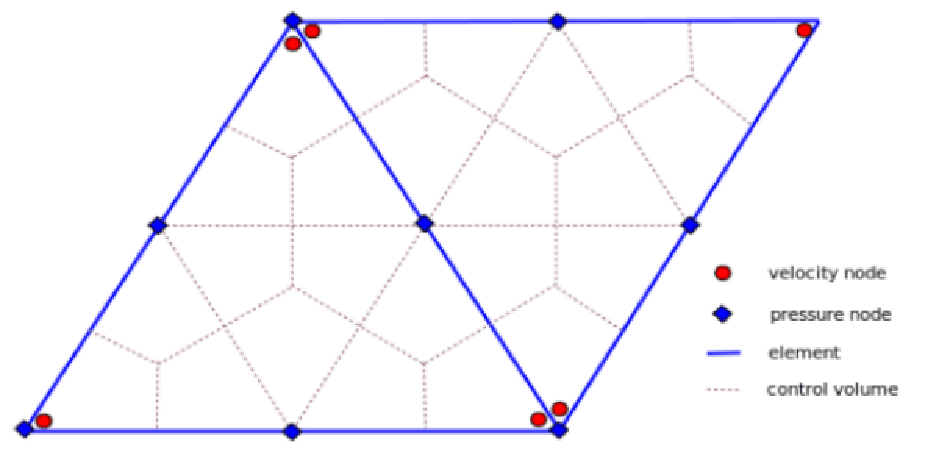
\includegraphics[width=0.75\linewidth, height=5cm]{./Pics/P1DG-P2_element_type} 
\caption{Caption 2}
\label{fig:2}
\end{center}

\begin{center}
\centering
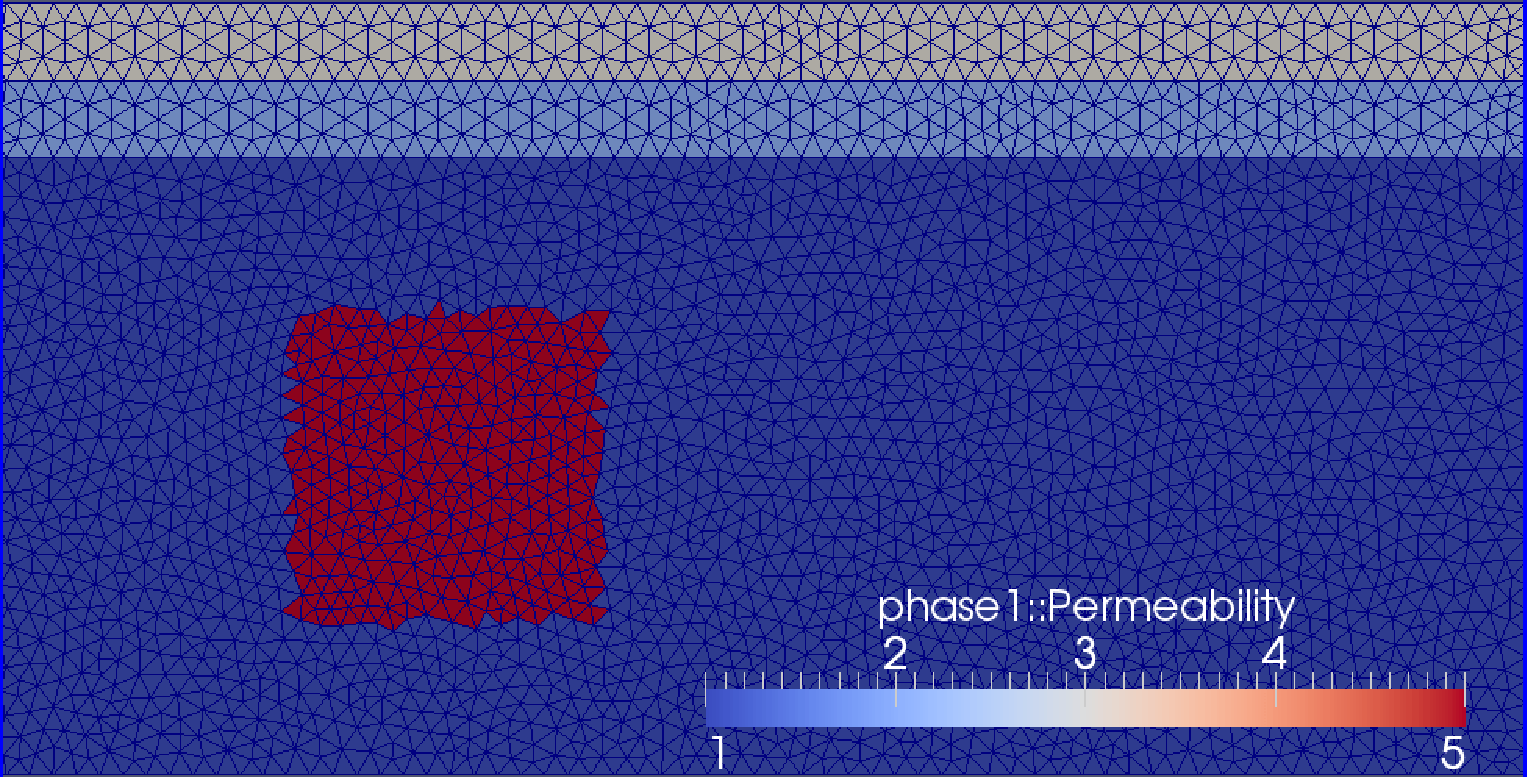
\includegraphics[width=0.8\linewidth, height=7cm]{./Pics/4r_po_adapt_fine_125_mesh} 
\caption{Caption 3}
\label{fig:3}
\end{center}

\begin{center}
\centering
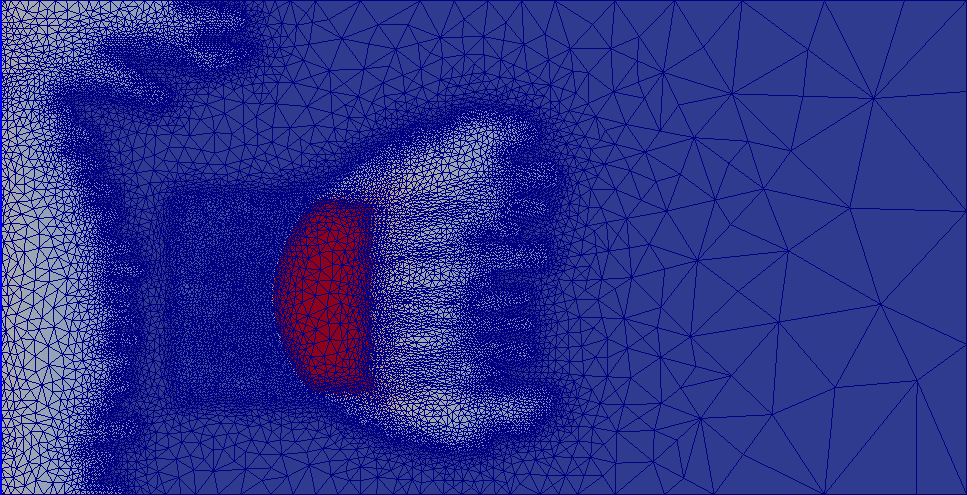
\includegraphics[width=0.8\linewidth, height=7cm]{./Pics/4r_po_adapt_fine_100_mesh}
\caption{Caption 4}
\label{fig:4}
\end{center}
 
%\caption{Caption for this figure with two images}
\label{fig:image2}
\end{figure}
\pagebreak
\clearpage

\begin{landscape}
\begin{figure}[ht!]
\begin{center}
\subfigure[MR100, at the beginning of the simulations]{%
\label{fig:1st}
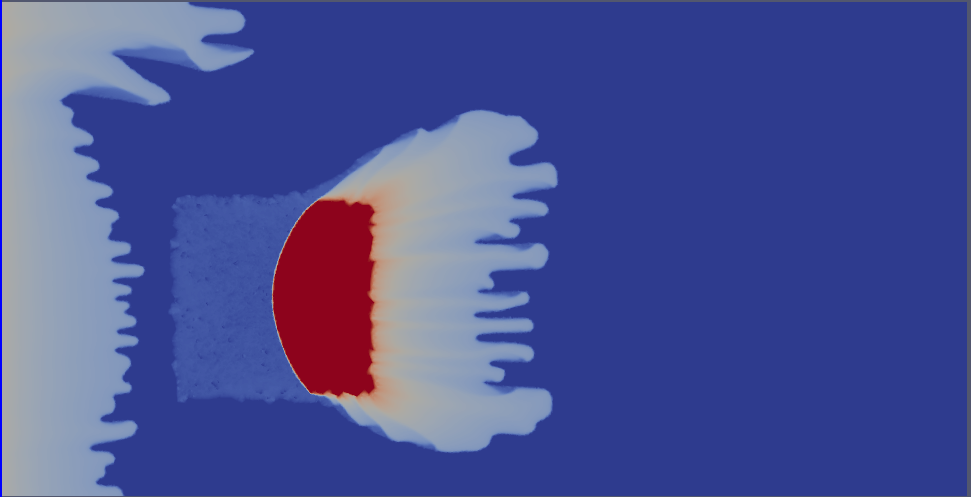
\includegraphics[width=0.75\textwidth]{./Pics/4r_po_adapt_fine_100}
}%
\subfigure[MR100, at the middle of the simulation]{%
\label{fig:2nd}
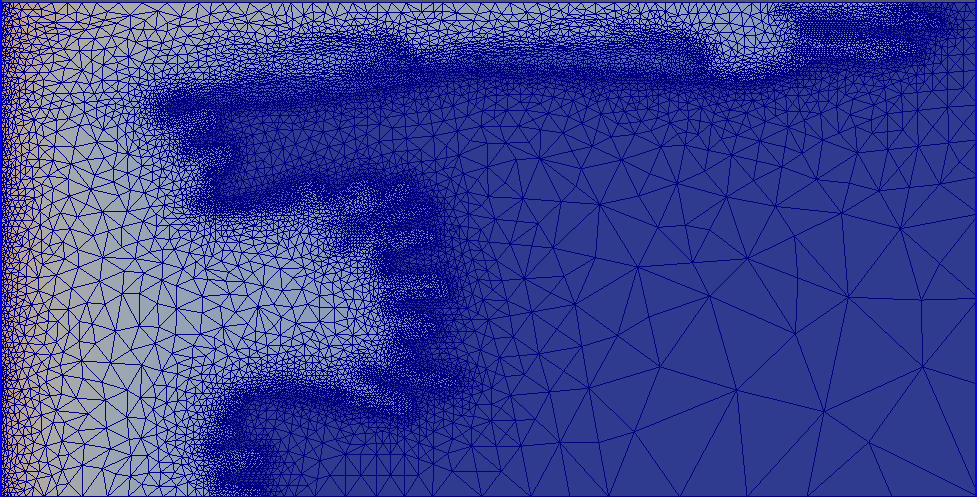
\includegraphics[width=0.75\textwidth]{./Pics/4r_po_adapt_fine_125_phase1_vol_fraction_mesh}
}\\
\subfigure[MR100, Phase 1 Volume fraction]{%
\label{fig:3rd}
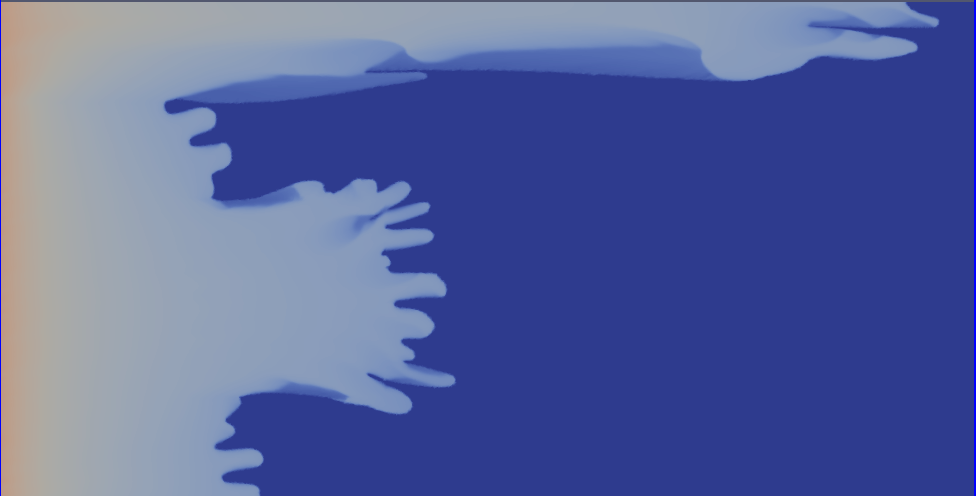
\includegraphics[width=0.75\textwidth]{./Pics/4r_po_adapt_fine_125_phase1_vol_frac}
}%
\subfigure[MR100, Phase 2 Volume fraction]{%
\label{fig:4th}
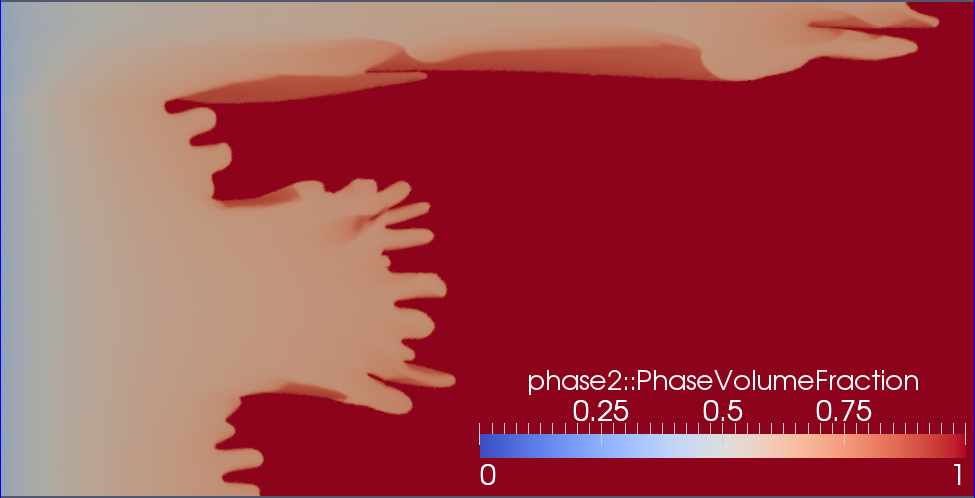
\includegraphics[width=0.75\textwidth]{./Pics/4r_po_adapt_fine_125_phase2_vol_fraction}
}\\
\caption{Comparison of different MR's and their recovery rates}
\label{fig:5}
\end{center}
\end{figure}
\end{landscape}

\pagebreak
\clearpage
%
%%%%
%%%%  FIGURE 
%%%%
\begin{figure}[h]
\centering
\vbox{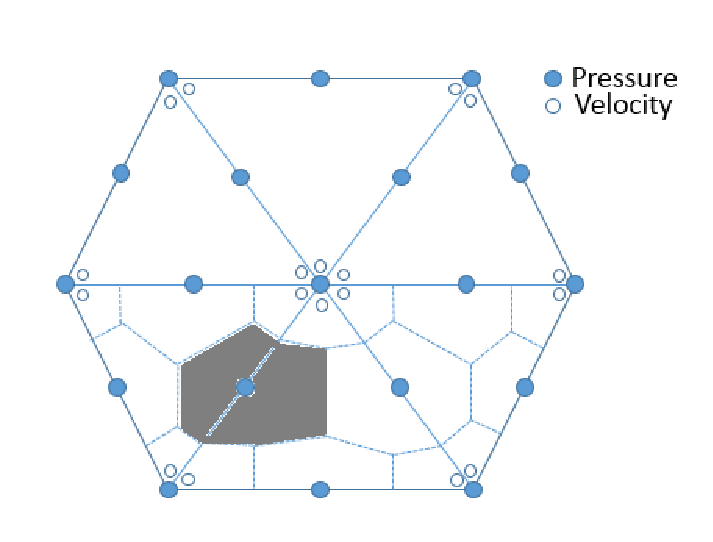
\includegraphics[width=.5\textwidth]{./Pics/P1DGP2.pdf}}
\caption{2D representation of \PN[1]{2} element pairs used in this work. Shaded areas denote control volumes across two contiguous elements. Blue and white circles represent pressure and velocity nodes, respectively.} 
\label{fig:fem_cv}
\end{figure}

\clearpage

%%%%
%%%%  FIGURE
%%%%
\begin{figure}[h]
\centering
\vbox{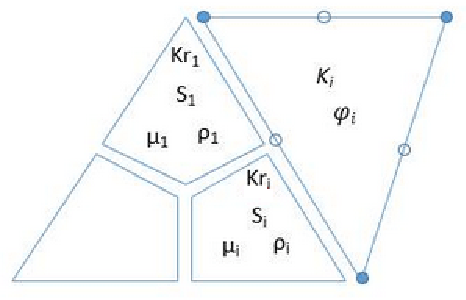
\includegraphics[width=.75\textwidth]{./Pics/element_n.pdf}}
\caption{This is a graphical representation of two different element types. Triangle {\it A} is a representation of the \PN[1]{2} element-pair, whereas triangle {\it B} represents the \PN[1]{1} element-pair. Porosity $\phi_{i}$, permeability {\bf K}$_{i}$, velocity and pressure are primarily represented in FE space whereas scalar fields (such as saturation, density, viscosity etc) are represented in CV space.}
\label{fig:fem_elem}
\end{figure}
\clearpage

%%%%
%%%%  FIGURE 
%%%%
\begin{figure}[h]
\centering
\vbox{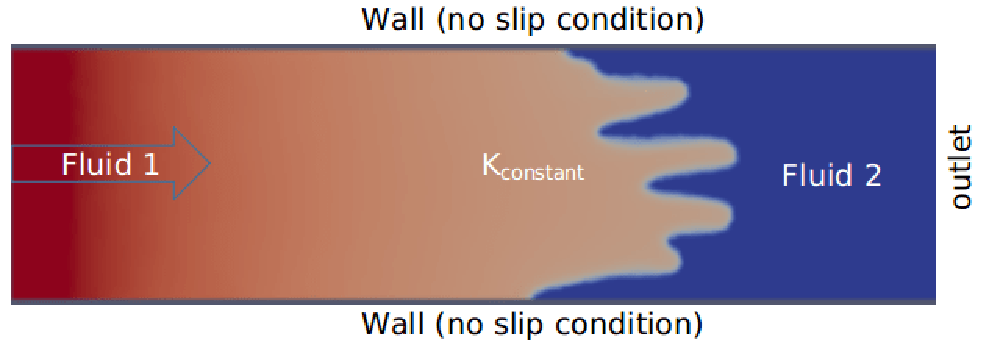
\includegraphics[width=0.75\textwidth]{./Pics/phase_vol_frac_uni_perm_1.pdf}}
\caption{Schematics of formation of flow instabilities during injection of a pure low viscosity fluid (red) into a domain saturated with a second fluid (dark blue). The ratio of viscosity between the two fluids is 5. In this case, the initially piston shape front collapses leading to the formation of several fingers.}
\label{fig:simple_case}
\end{figure}
\clearpage


%%%%
%%%%  FIGURE 
%%%%
\begin{figure}[ht] 
\vbox{
\hbox{\hspace{-0.3cm}
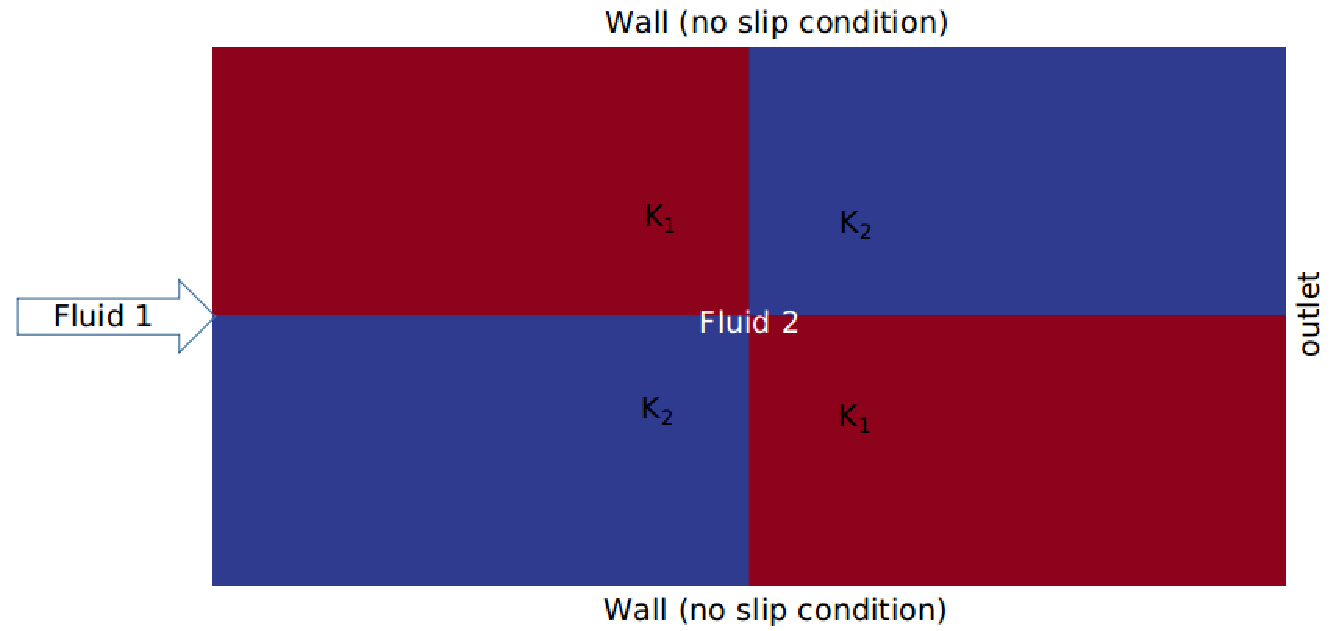
\includegraphics[width=.8\textwidth]{./Pics1/2b2_wi_fine/2b2_whole_in_fine_perm_1.pdf} 
}
\vspace{0.0cm}
\hbox{\hspace{3.5cm} (a) map of permeabilities ($\mathbf{K}$)
}
\vspace{0.25cm}
\hbox{\hspace{1.5cm}
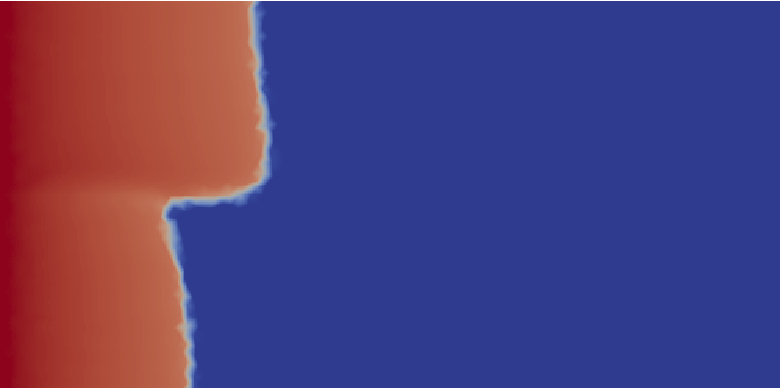
\includegraphics[width=.85\textwidth]{./Pics1/2b2_wi_fine/2b2_whole_in_fine_250_2.pdf}
}
\vspace{0.0cm}
\hbox{\hspace{4.5cm} (b) flow at t=250 
}
\vspace{0.25cm}
\hbox{\hspace{1.5cm}
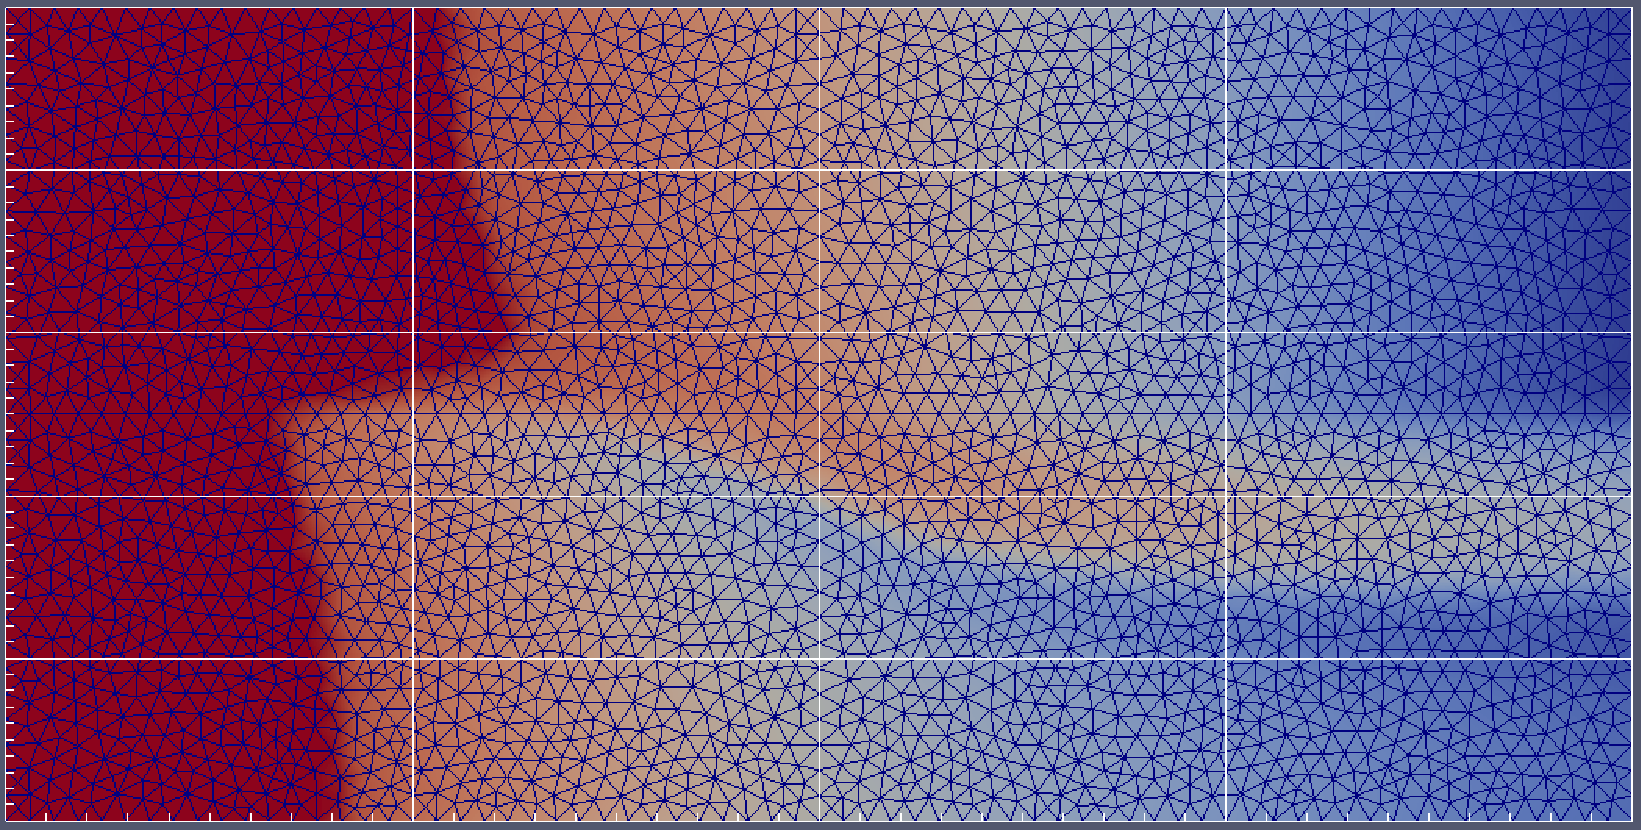
\includegraphics[width=.65\textwidth]{./Pics1/2b2_wi_fine/2b2_whole_in_fine_3000_2.pdf}
}
\vspace{0.0cm}
\hbox{\hspace{4.0cm} (c) flow at t=3000   
}}     
\caption{Model validation of fluid displacement in heterogeneous porous media ({\it VR}=1): (a) the domain is divided into four subdomains with prescribed synthetic permeability, $\mathbf{K}_{1}=1$ and $\mathbf{K}_{2}=2.5$; (b-c) snapshots of saturation (displacing fluid) field at t=$25$s and t=$300$ sec. The domain is discretised with $5960$ \PN[1]{2} elements. }
\label{fem_cv_represent_a}
\end{figure}
\clearpage



%%%%
%%%%  FIGURE
%%%%
\begin{landscape}
\begin{figure}[ht] 
\vbox{\vspace{-1cm}
\hbox{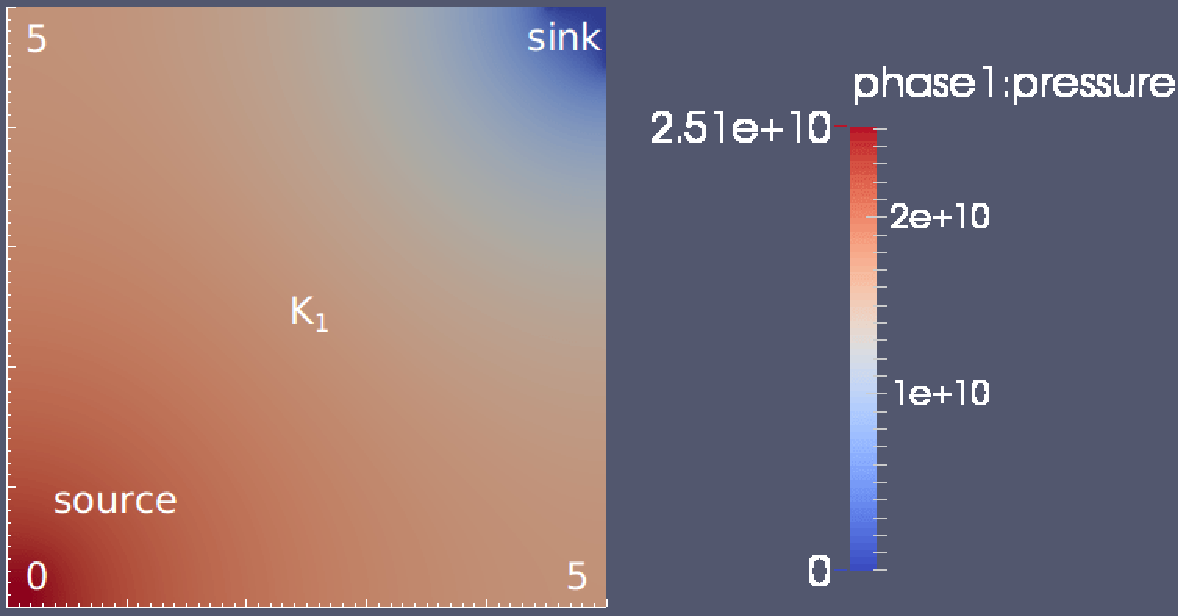
\includegraphics[width=.7\textwidth]{./Pics1/Saffman_homogeneous_MR3/saffman_homo_fixed_2.pdf}
      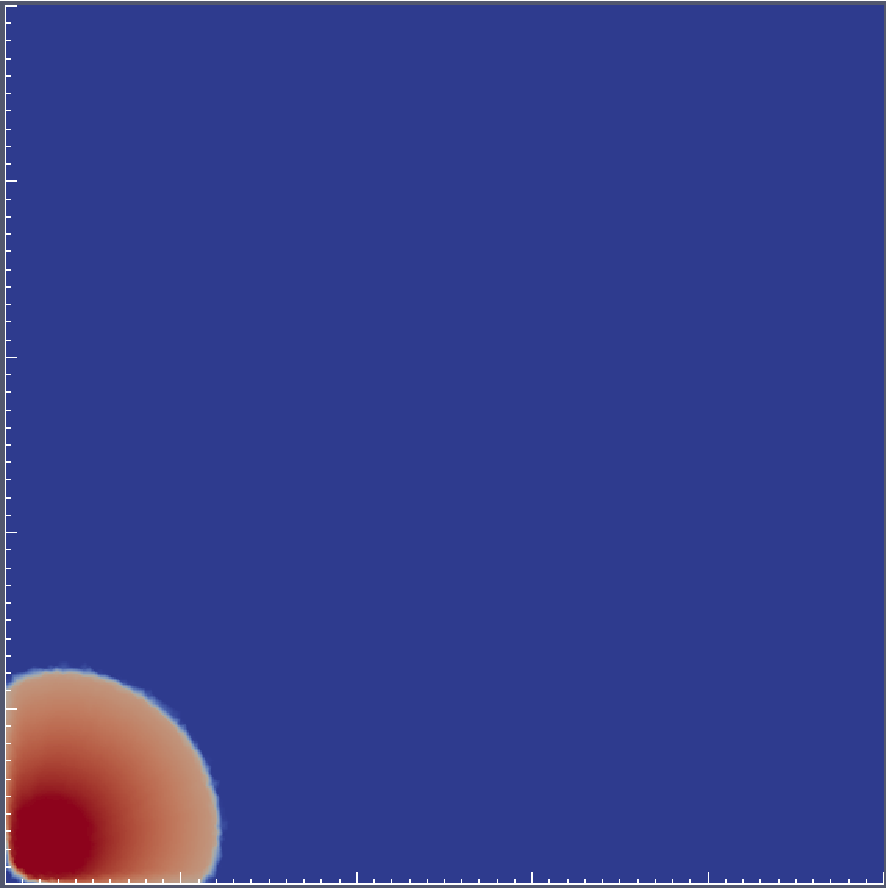
\includegraphics[width=.37\textwidth]{./Pics1/Saffman_homogeneous_MR3/saffman_homo_fixed_250.pdf}
      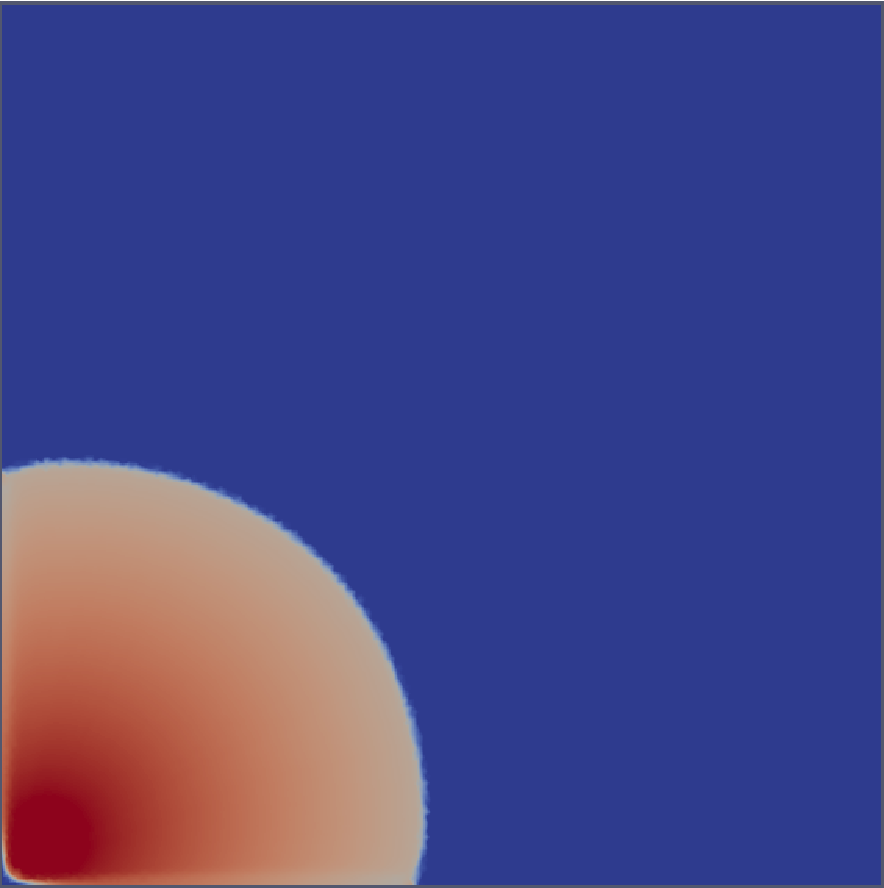
\includegraphics[width=.37\textwidth]{./Pics1/Saffman_homogeneous_MR3/saffman_homo_fixed_1000.pdf}}
\vspace{0.cm}
\hbox{\hspace{2.5cm} (a) pressure at t=0s \hspace{5.cm} (b) t=0.87s \hspace{2.75cm} (c) t=3.54s}
\vspace{0.5cm}
\hbox{
      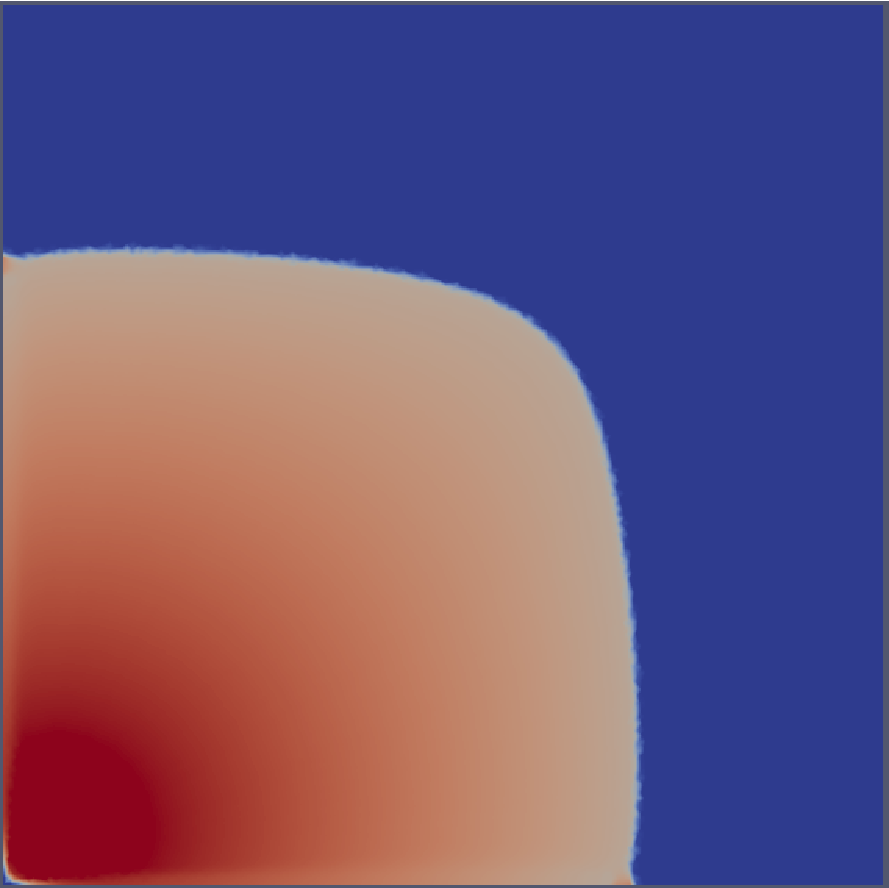
\includegraphics[width=.375\textwidth]{./Pics1/Saffman_homogeneous_MR3/saffman_homo_fixed_2500.pdf}
      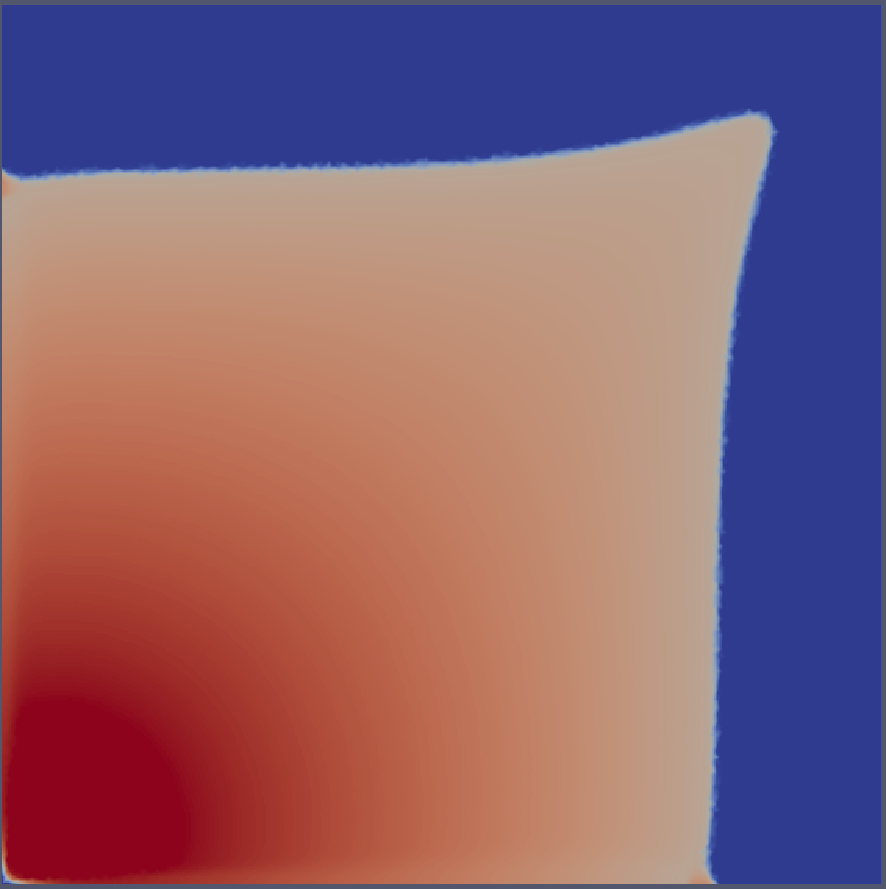
\includegraphics[width=.375\textwidth]{./Pics1/Saffman_homogeneous_MR3/saffman_homo_fixed_3500.pdf} 
      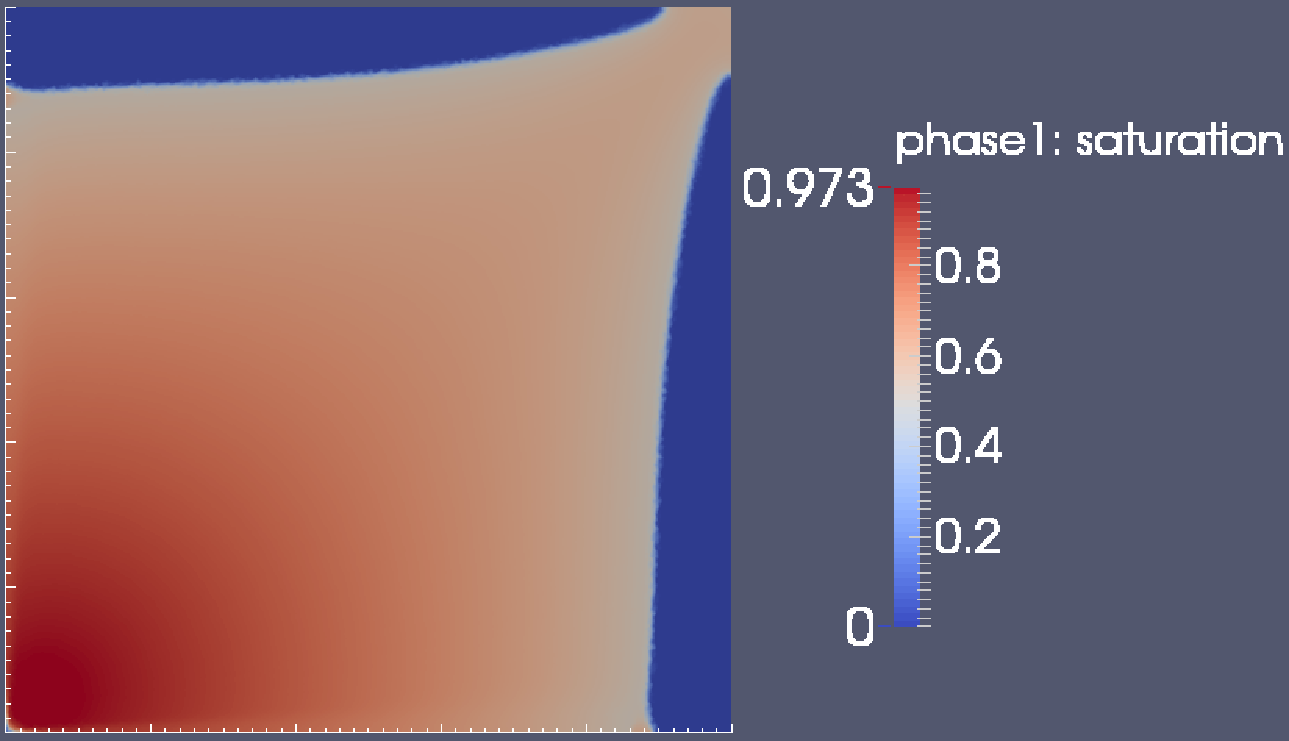
\includegraphics[width=.65\textwidth]{./Pics1/Saffman_homogeneous_MR3/saffman_homo_fixed_end.pdf}}
\vspace{0.cm}
\hbox{ \hspace{1.cm} (d) t=8.86s \hspace{3.0cm} (e) t=12.41s   \hspace{4.0cm} (f) t=17.95s}
\vspace{0.cm}
}   
\caption{Simulated flow in a Hele-Shaw cell ({\it VR}=3): (a) initial pressure profile $\left(\text{in g.cm}^{-1}\text{.s}^{-2}\right)$ with source and sink regions are explicitly shown along with dimensions (in cm); (b-f) snapshots of wetting phase saturation showing flow profile as the simulation evolves. The domain contains $47500$ \PN[1]{2} triangular elements.}
\label{fig:homoheleshaw_VN3}
\end{figure}
\end{landscape}
\clearpage



%%%%
%%%%  FIGURE
%%%%
\begin{landscape}
\begin{figure}[ht] 
\vbox{\vspace{-1cm}
\hbox{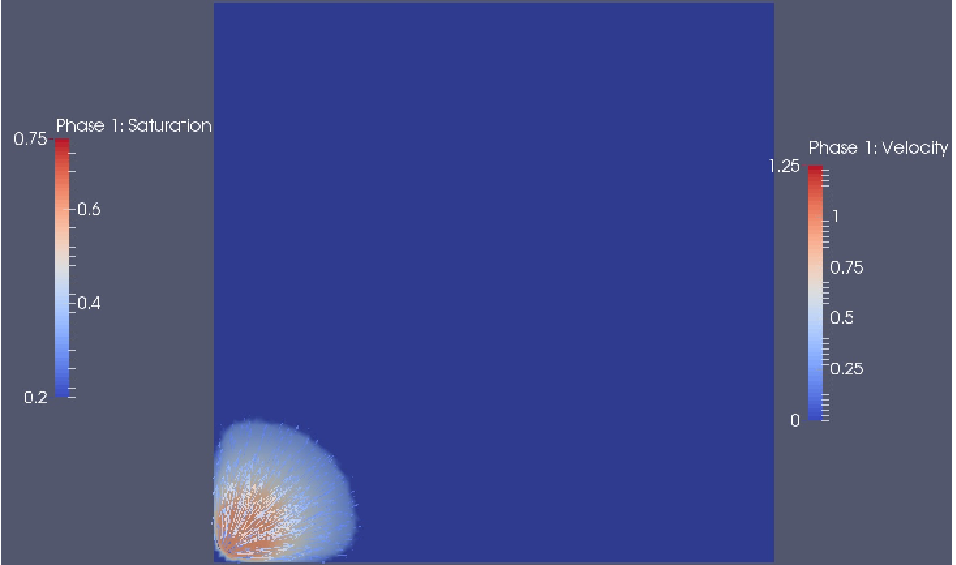
\includegraphics[width=.9\textwidth, height=0.5\textwidth]{./Pics1/Saffman_homogeneous_VR10/ST_Homog_VR10_D201c.pdf}
\hspace{0.5cm}      
      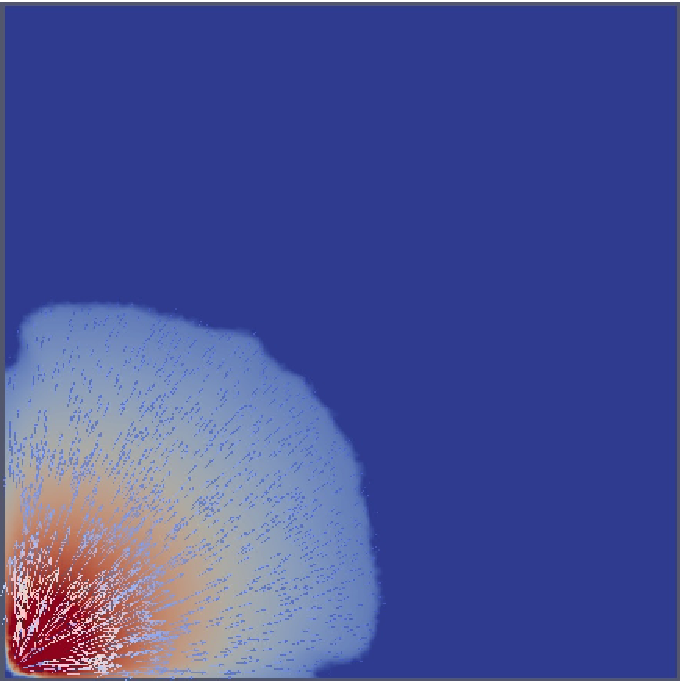
\includegraphics[width=.5\textwidth]{./Pics1/Saffman_homogeneous_VR10/ST_Homog_VR10_D1001c.pdf}}
\vspace{0.cm}
\hbox{\hspace{5.cm} (a) t=0.66s \hspace{8.cm} (b) t=3.43s }
\vspace{0.5cm}
\hbox{
      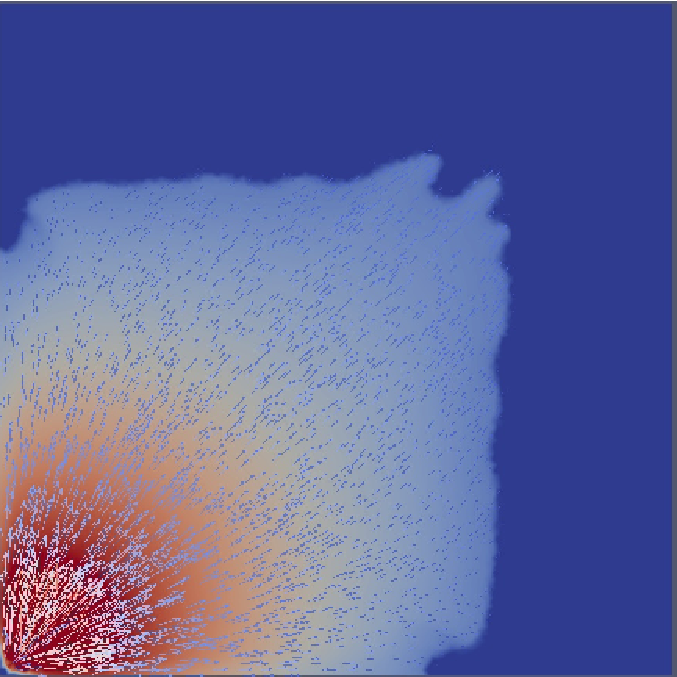
\includegraphics[width=.5\textwidth]{./Pics1/Saffman_homogeneous_VR10/ST_Homog_VR10_D2001c}
      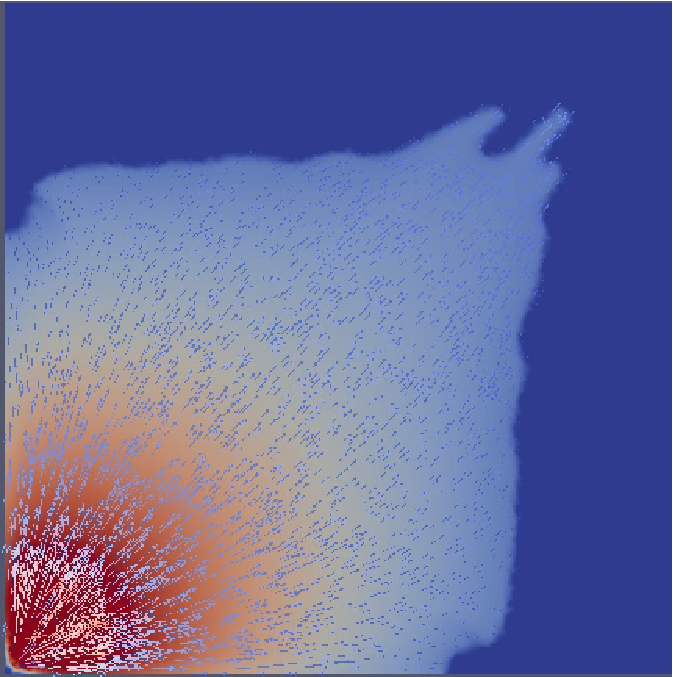
\includegraphics[width=.5\textwidth]{./Pics1/Saffman_homogeneous_VR10/ST_Homog_VR10_D2201c}
      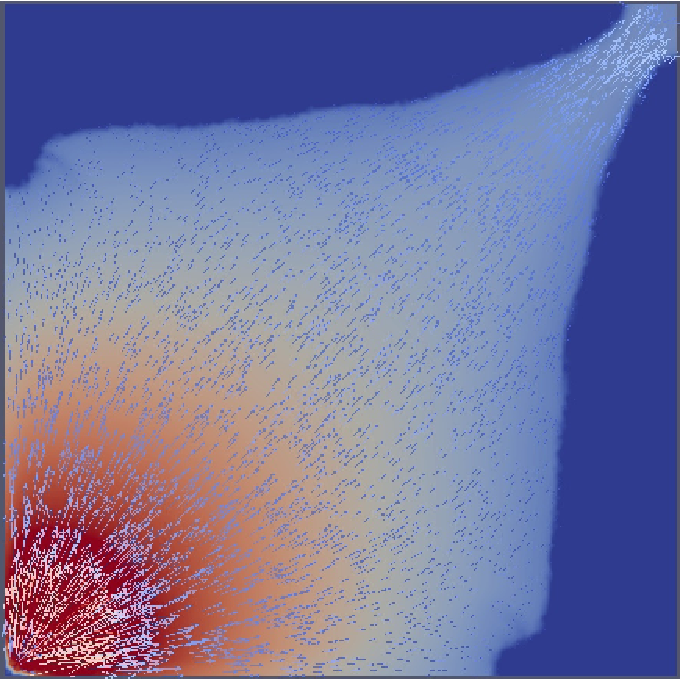
\includegraphics[width=.5\textwidth]{./Pics1/Saffman_homogeneous_VR10/ST_Homog_VR10_D3001c}}
\vspace{0.cm}
\hbox{ \hspace{2.cm} (c) t=6.92s \hspace{4.5cm} (d) t=7.61s \hspace{4.5cm} (e)t=10.00s}
\vspace{0.cm}
}   
\caption{Simulated flow in a Hele-Shaw cell ({\it VR}=10): snapshots of overlapped wetting phase saturation and velocity vectors showing flow profile as the simulation evolves. The domain contains $26313$ \PN[1]{2} triangular elements.}
\label{fig:homoheleshaw_VN10}
\end{figure}
\end{landscape}
\clearpage

%%%%
%%%%  FIGURE
%%%%
\begin{landscape}
\begin{figure}[ht] 
\vbox{\vspace{-1cm}
\hbox{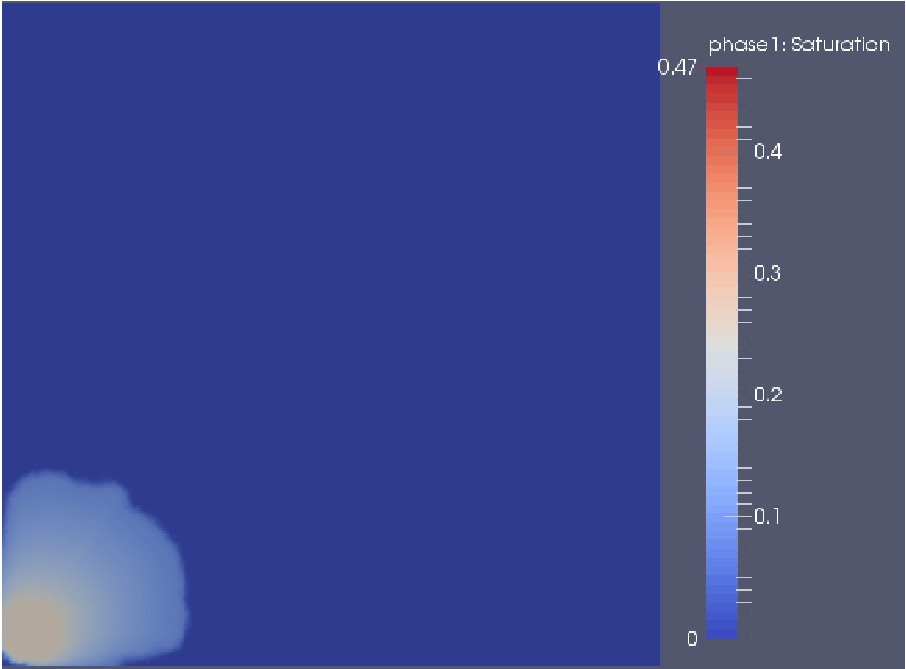
\includegraphics[width=.9\textwidth, height=0.5\textwidth]{./Pics1/Saffman_homogeneous_VR150/ST_Homog_VR150_D300b}
\hspace{0.5cm}      
      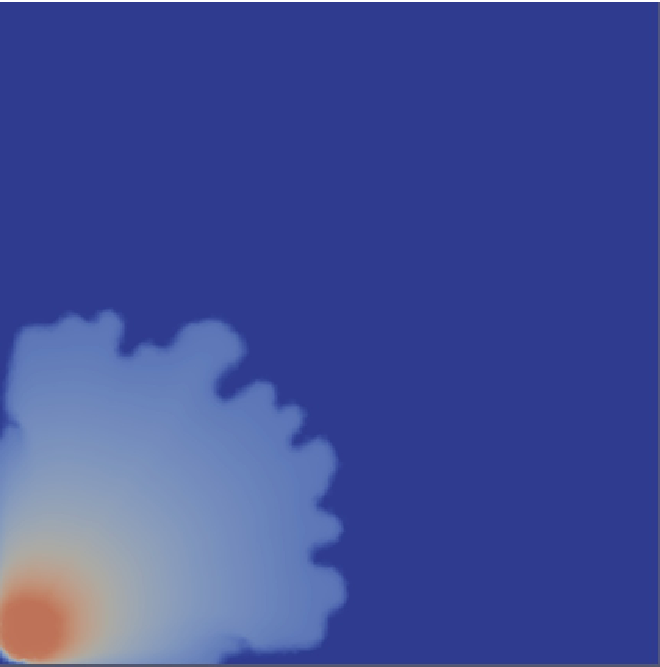
\includegraphics[width=.5\textwidth]{./Pics1/Saffman_homogeneous_VR150/ST_Homog_VR150_D1600b}}
\vspace{0.cm}
\hbox{\hspace{5.cm} (a) t=0.27s \hspace{8.cm} (b) t=0.94s }
\vspace{0.5cm}
\hbox{
      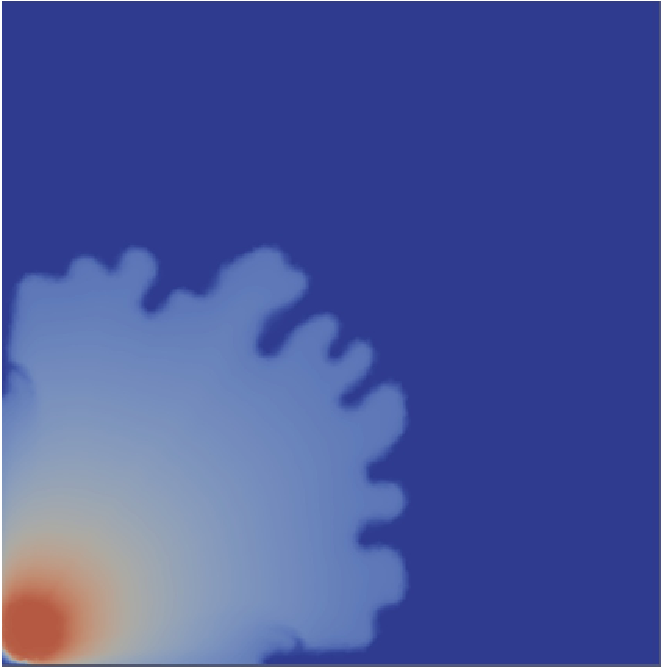
\includegraphics[width=.5\textwidth]{./Pics1/Saffman_homogeneous_VR150/ST_Homog_VR150_D2700b}
      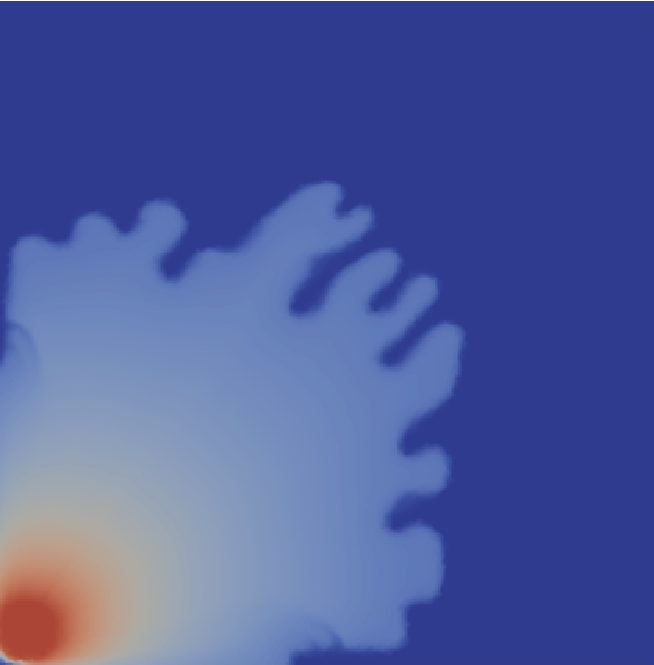
\includegraphics[width=.5\textwidth]{./Pics1/Saffman_homogeneous_VR150/ST_Homog_VR150_D4000b}
      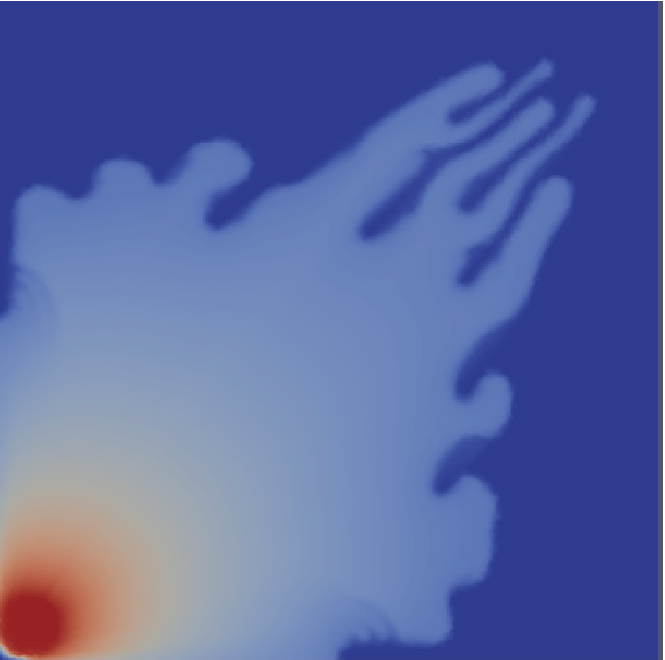
\includegraphics[width=.5\textwidth]{./Pics1/Saffman_homogeneous_VR150/ST_Homog_VR150_D7000b}}
\vspace{0.cm}
\hbox{ \hspace{2.cm} (c) t=1.32s \hspace{4.5cm} (d) t=1.70s \hspace{4.5cm} (e)t=2.31s}
\vspace{0.cm}
}   
\caption{Simulated flow in a Hele-Shaw cell ({\it VR}=150): snapshots of wetting phase saturation showing flow profile as the simulation evolves. The domain contains $26313$ \PN[1]{2} triangular elements.}
\label{fig:homoheleshaw_VN10}
\end{figure}
\end{landscape}
\clearpage


%%%%
%%%%  FIGURE
%%%%
\begin{landscape}
\begin{figure}[ht] 
\hbox{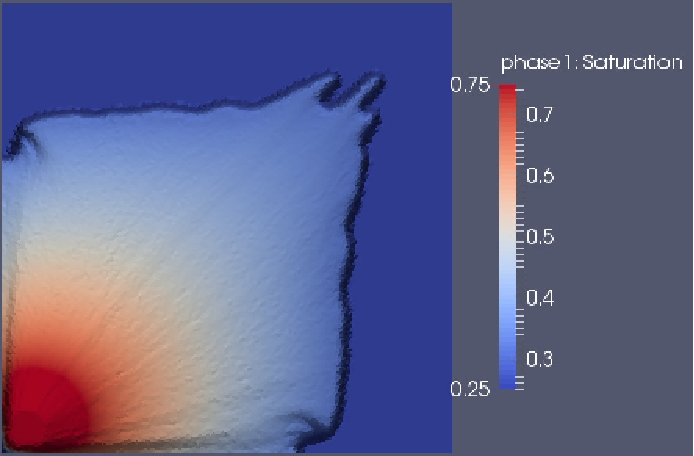
\includegraphics[width=.5\textwidth]{./Pics1/Saffman_homogeneous_VR10/ST_Homog_VR10_D2201_bbd}
       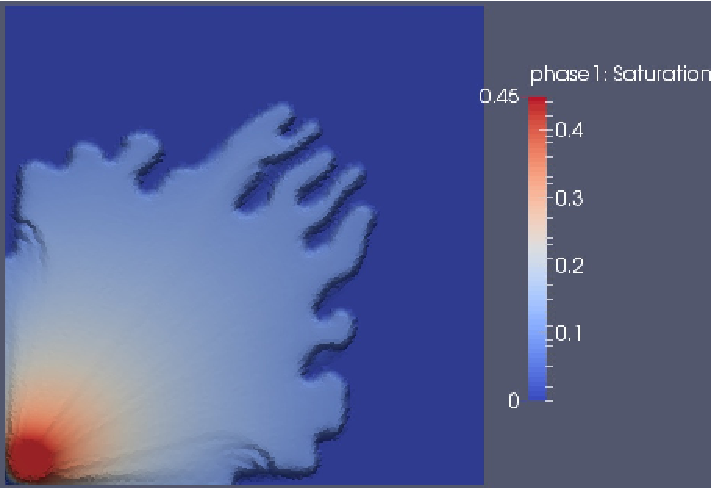
\includegraphics[width=.49\textwidth]{./Pics1/Saffman_homogeneous_VR150/ST_Homog_VR150_D5003_k2b}}
\caption{Simulated flow in Hele-Shaw cells performed with viscosity ratios of 10 (left, t=7.61s) and 150 (t=1.94s). Width of largest fingers are approximetely 0.70 and 0.90cm, which are in good agreement with values obtained from \citet{guan_2003}'s analytic solution. Domains of both simulations contain $26313$ \PN[1]{2} triangular elements.\red{(More pics to be added!!)}}
\label{fig:homoheleshaw_VN10_VN150}
\end{figure}
\end{landscape}



\begin{comment}

%%%%
%%%%  FIGURE
%%%%
\begin{landscape}
\begin{figure}[ht] 
\vbox{\vspace{-1cm}
\hbox{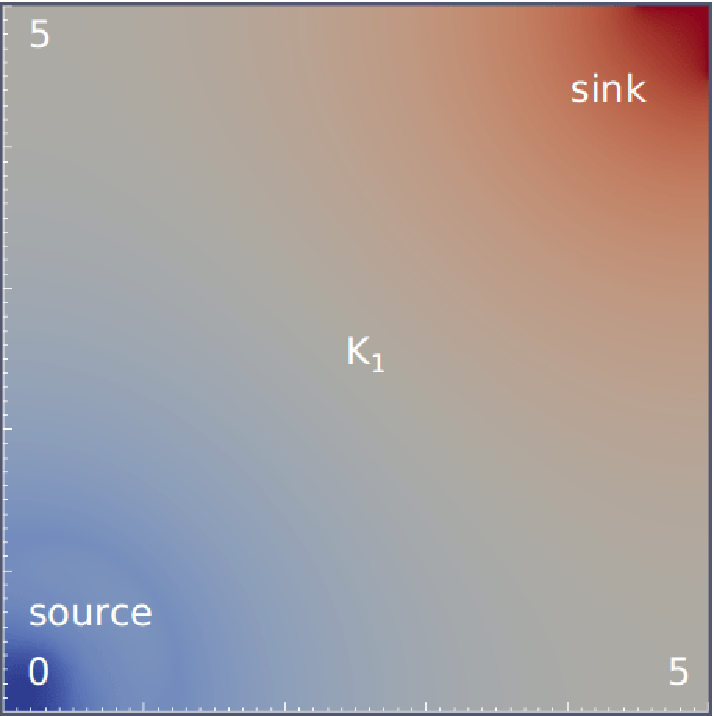
\includegraphics[width=.5\textwidth]{./Pics1/Saffman_homogeneous/saffman_homo_fixed_1.pdf}
      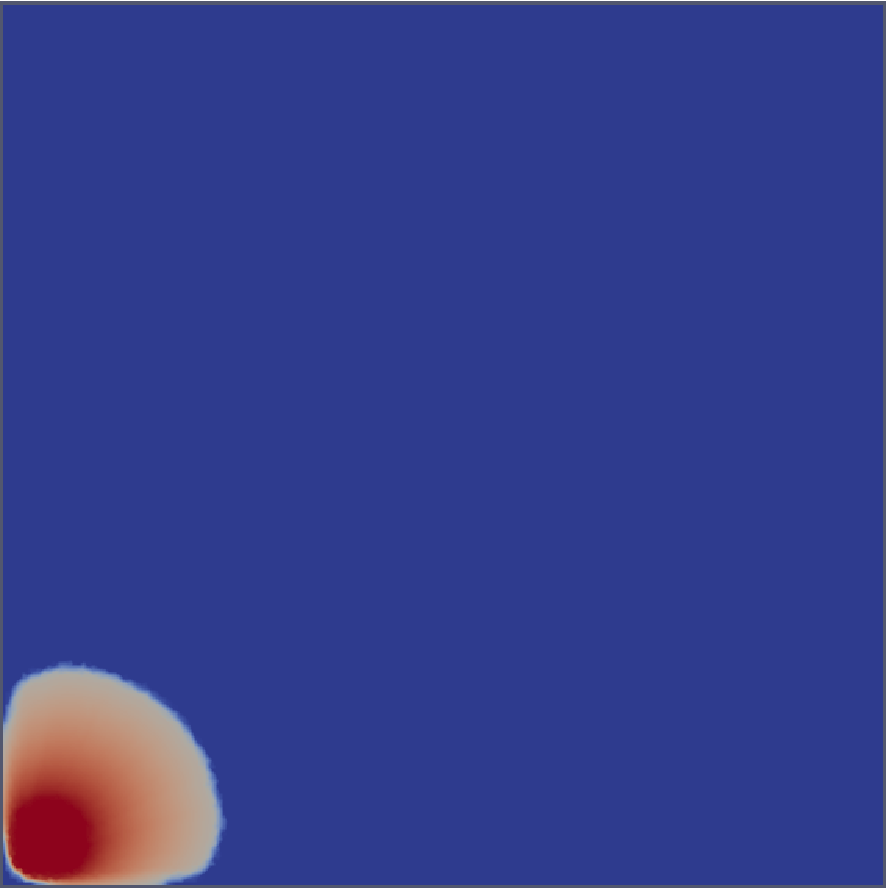
\includegraphics[width=.5\textwidth]{./Pics1/Saffman_homogeneous/saffman_homo_fixed_250_1.pdf}
      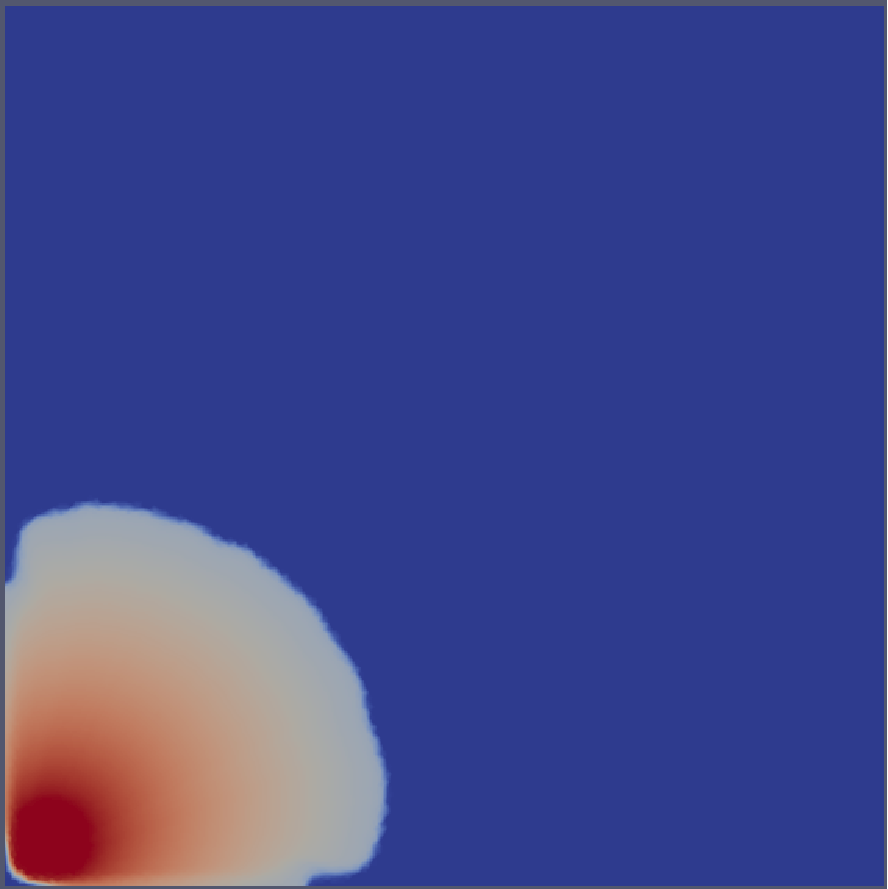
\includegraphics[width=.5\textwidth]{./Pics1/Saffman_homogeneous/saffman_homo_fixed_1000.pdf}}
\vspace{0.cm}
\hbox{\hspace{1.0cm} (a) pressure at t=0 \hspace{3.cm} (b) t=250\red{(???)} \hspace{3.0cm} (c) t=1000\red{(???)}}
\vspace{0.5cm}
\hbox{
      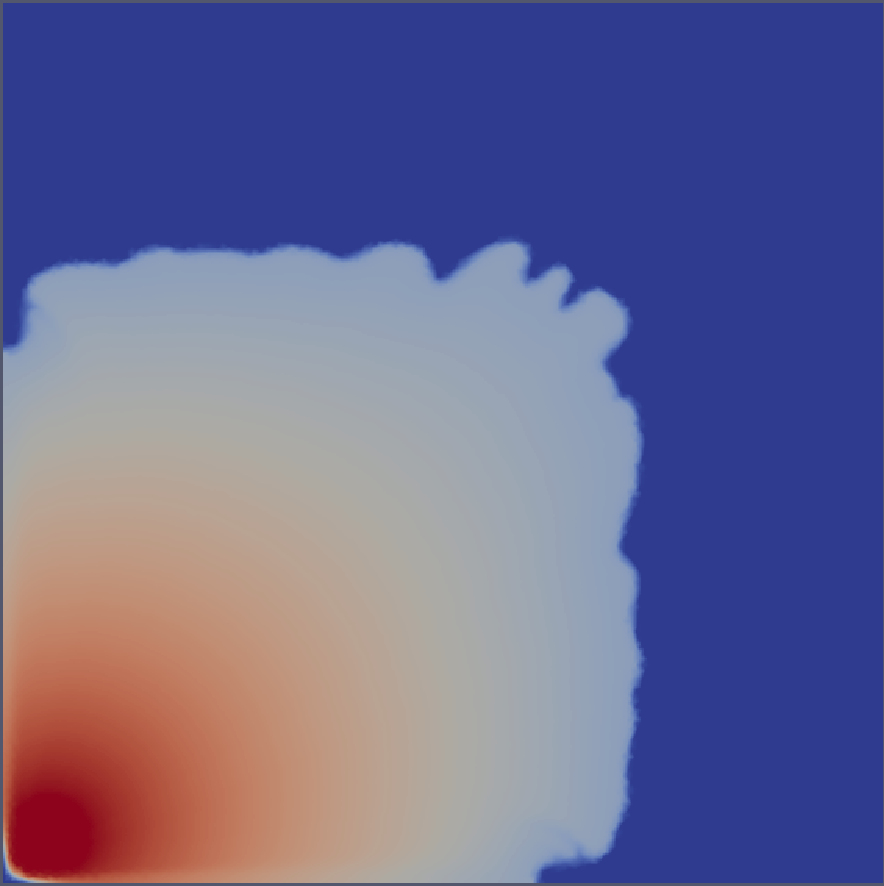
\includegraphics[width=.5\textwidth]{./Pics1/Saffman_homogeneous/saffman_homo_fixed_6000.pdf}
      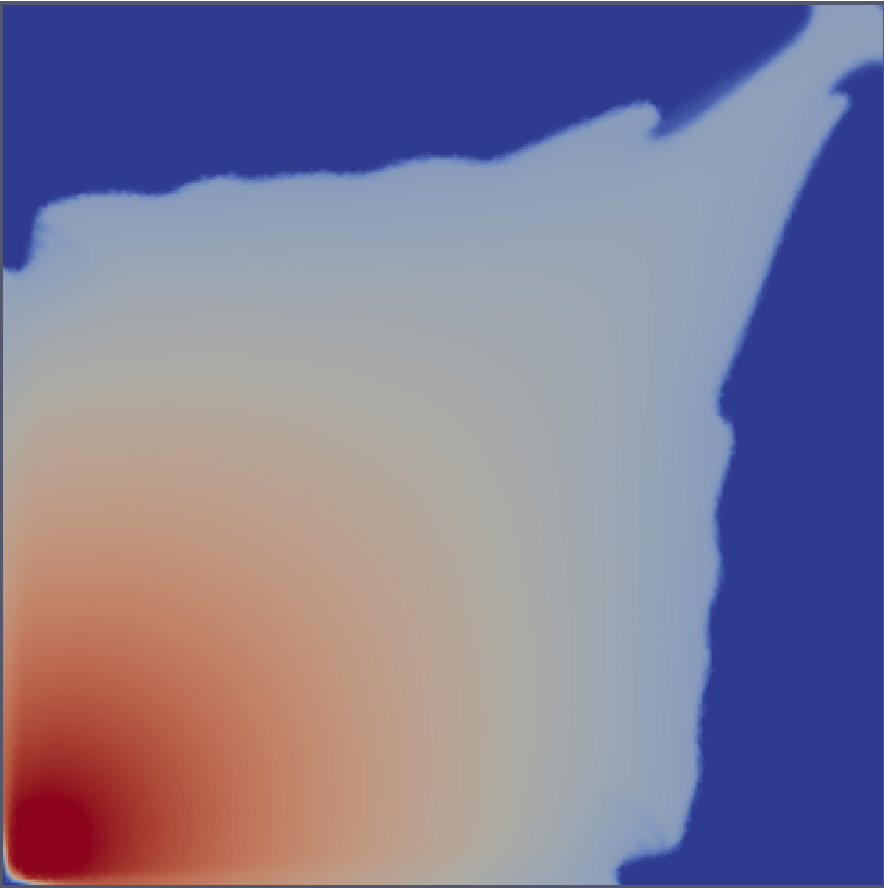
\includegraphics[width=.5\textwidth]{./Pics1/Saffman_homogeneous/saffman_homo_fixed_end_1.pdf}}
\vspace{0.cm}
\hbox{ \hspace{2.cm} (d) t=6000\red{(???)} \hspace{3.cm} (e) t=XXX\red{(???)}}
\vspace{0.cm}
}   
\caption{Simulated flow in a Hele-Shaw cell ({\it VR}=10): (a) pressure profile $\left(\text{in g.cm}^{-1}\text{.s}^{-2}\right)$ with source and sink regions explicitly shown along with dimensions (in cm); (b-e) snapshots of wetting phase saturation showing flow profile as the simulation evolves. The domain contains $47000$ \PN[1]{2} triangular elements. The pressure and saturation range of values are the same like the  case in fig.\ref{fig:homoheleshaw_VN3}.}
\label{fig:homoheleshaw_VN10}
\end{figure}
\end{landscape}
\clearpage
\end{comment}


%%%
%%% FIGURE XXXXXX
%%%
\begin{landscape}
  \begin{figure}[ht]
  \vbox{\vspace{-1cm}
      \hbox{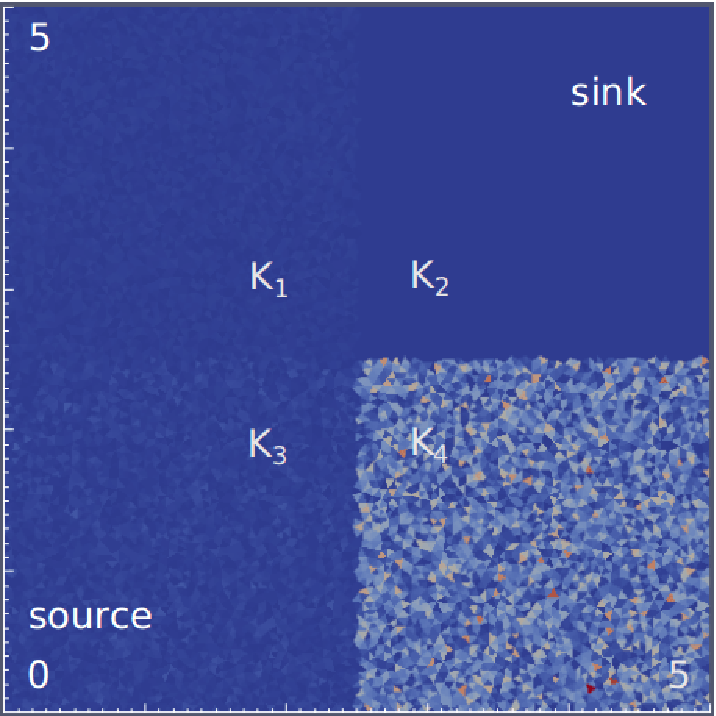
\includegraphics[width=.5\textwidth]{./Pics1/Saffman_heterogeneous/saffman_heter_fixed_1.pdf}
            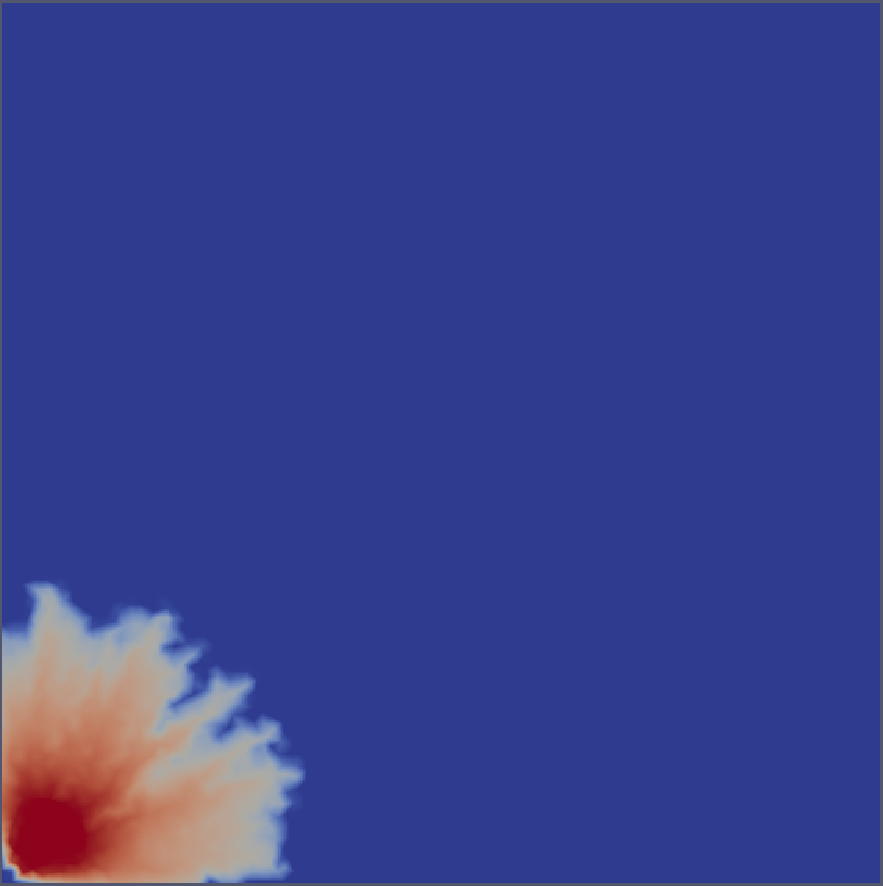
\includegraphics[width=.5\textwidth]{./Pics1/Saffman_heterogeneous/saffman_heter_fixed_500.pdf} 
            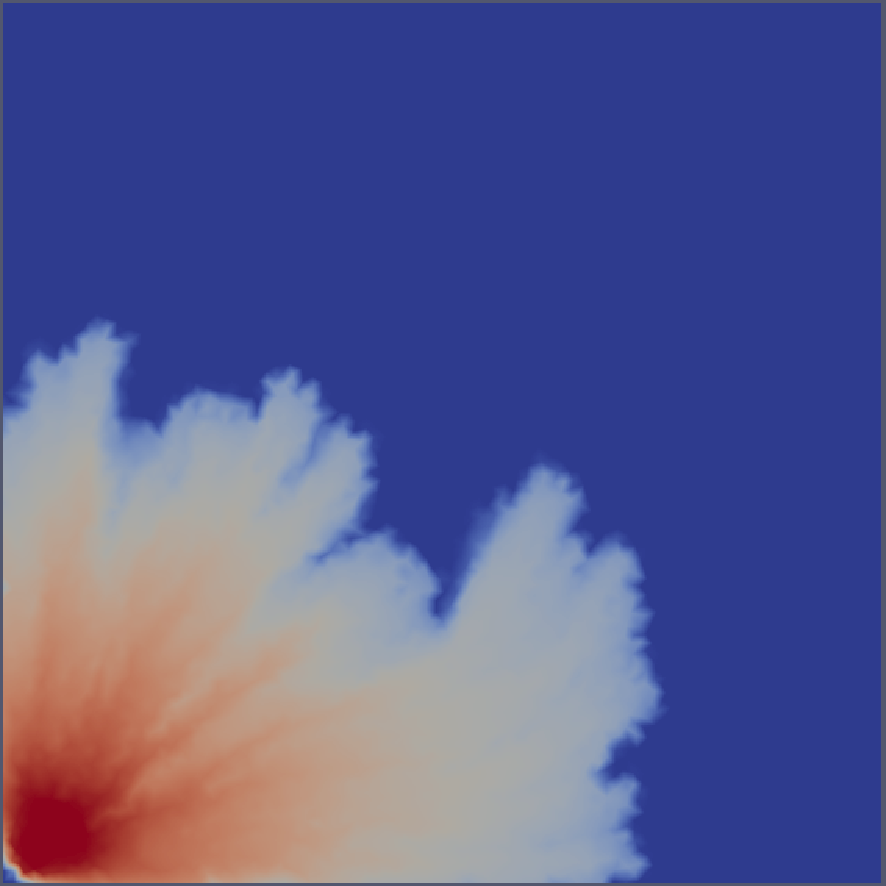
\includegraphics[width=.5\textwidth]{./Pics1/Saffman_heterogeneous/saffman_heter_fixed_2000.pdf} }
      \hbox{\hspace{1.0cm} (a) permeability map \hspace{3.cm} (b) t=0.75s \hspace{4.0cm} (c) t=8s}
      \vspace{0.5cm}
      \hbox{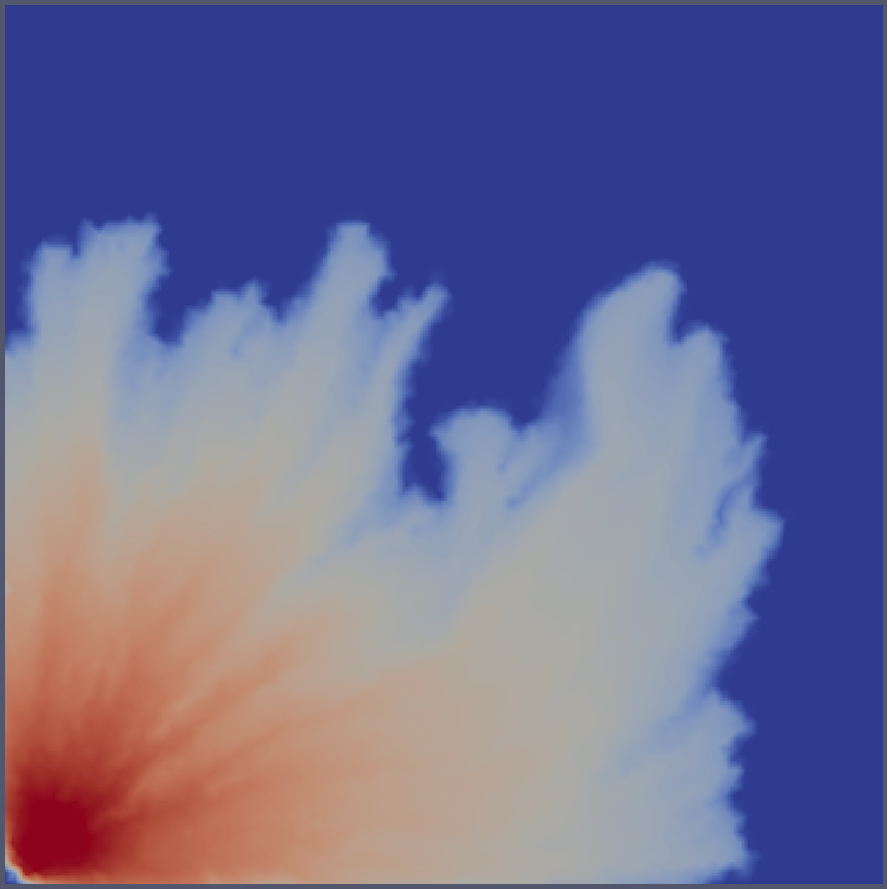
\includegraphics[width=.5\textwidth]{./Pics1/Saffman_heterogeneous/saffman_heter_fixed_3000.pdf}
            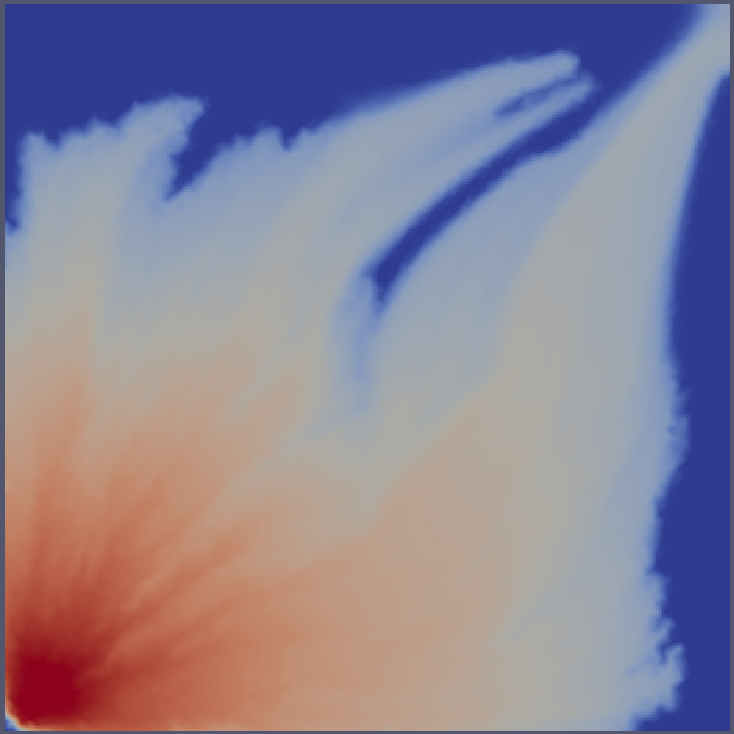
\includegraphics[width=.5\textwidth]{./Pics1/Saffman_heterogeneous/saffman_heter_fixed_6000.pdf}
            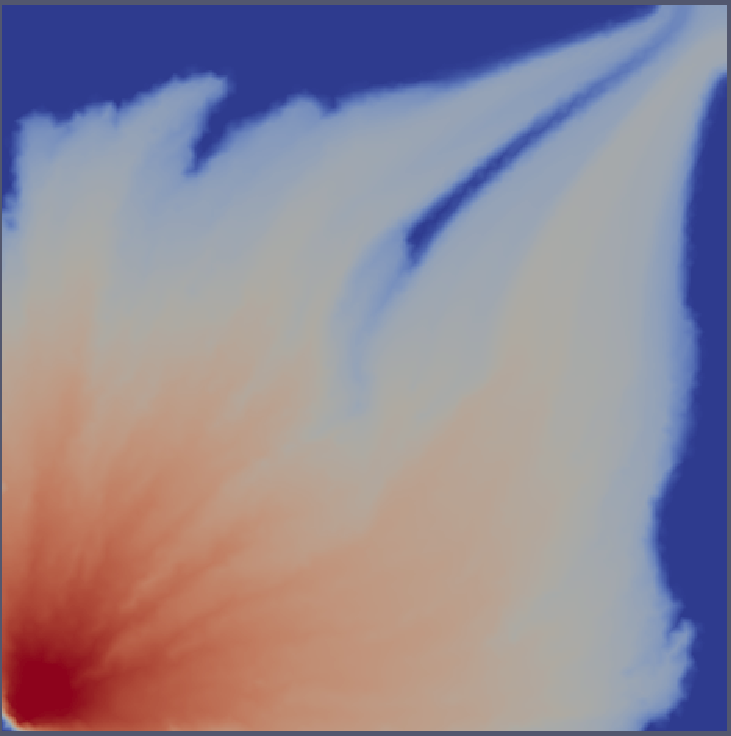
\includegraphics[width=.5\textwidth]{./Pics1/Saffman_heterogeneous/saffman_heter_fixed_24000.pdf} }
      \hbox{\hspace{2.5cm} (d) t=18s \hspace{5.cm} (e) t= \hspace{3.0cm} (f) t=24000 }}
\caption{Simulated flow in a modified Hele-Shaw cell with {\it VR}=10: (a) permeability distribution $\left(\text{10}^{-10}\le\mathbf{K}_{1}\le\text{5}\times\text{10}^{-10}\right.$, {\bf K}$_{2}$=10$^{-10}$, 10$^{-11}\le\mathbf{K}_{3}\le$ 5$\times$10$^{-10}$ and 10$^{-12}\le\mathbf{K}_{4}\le$ 5$\times$10$\left.^{-10}\text{ cm}^{2}\right)$; (b-f) snapshots of saturation profile during \red{XX} seconds of simulation. The domain contains \red{XX} \PN[1]{2} element-pairs.}
\label{fig:HeleShawHeter_VR10}
\end{figure}
\end{landscape}
\clearpage



%%%%
%%%%  FIGURE
%%%%
\begin{landscape}
\begin{figure}[ht] 
\vbox{
\hbox{\hspace{4.0cm}
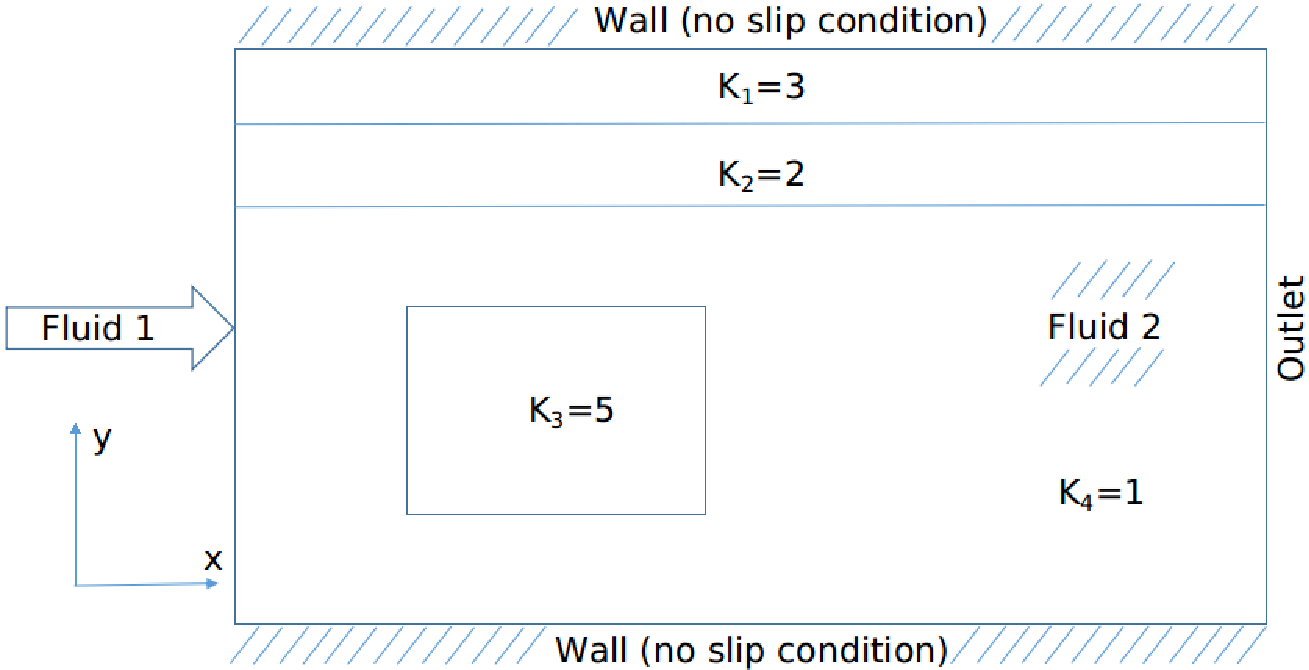
\includegraphics[width=.75\textwidth]{./Pics/map_of_boundaries.pdf} 
}
\vspace{0.0cm}
\hbox{\hspace{6.5cm} (a) map of permeabilties K   
}
\vspace{0.25cm}
\hbox{\hspace{4.0cm}
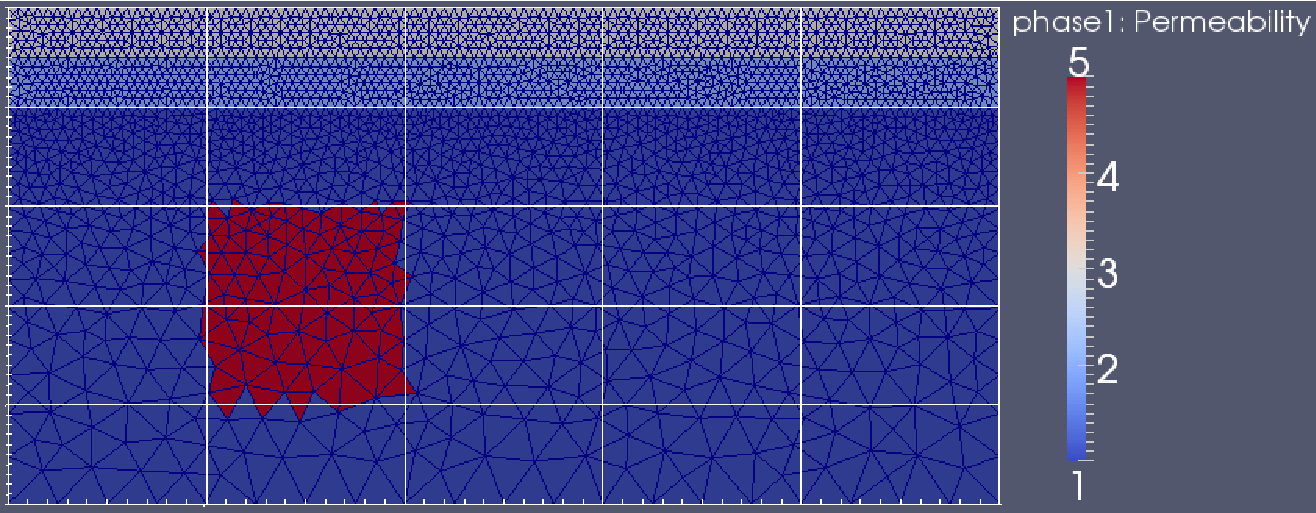
\includegraphics[width=.9\textwidth]{./Pics/map_of_boundaries_1.pdf}
}
\vspace{0.0cm}
\hbox{\hspace{9cm} (b)      
}
}     
\caption{Figure (a) describes the initial and boundary conditions as these are applied in this set of simulations. Below (b) there is a comparison between the unstructured and fixed mesh and the unstructured and adaptive mesh. During the implementation of fixed mesh initially there $4606$ elements while for the adaptive mesh there are $606$ while the majority of them is on the interface between between the two fluids. }
\label{fig:testcase_heter_domain}
\end{figure}
\end{landscape}
\clearpage



%%%%
%%%%  FIGURE
%%%%
\begin{landscape}
\begin{figure}[ht] 
\vbox{
\hbox{\hspace{3.5cm}
\includegraphics[width=.65\textwidth]{./Pics1/mr10_5regions_fixed/5regions_fixed_250.pdf} 
}
\vspace{0.0cm}
\hbox{\hspace{6.5cm} (a) flow at t=250 (fixed mesh)  
}
\vspace{0.25cm}
\hbox{\hspace{3.5cm}
\includegraphics[width=.9\textwidth]{./Pics1/mr10_5regions_adapt/5regions_adapt_250_1.pdf}
}
\vspace{0.0cm}
\hbox{\hspace{6.5cm} (b) flow at t=250 (adaptive mesh)    
}
}     
\caption{For $t=0.125$s, $2$ test-cases under the VR=$10$ and under fixed (top) and adaptive(bottom) mesh are compared. There is a significant difference on the main front (left hand side of the domain) and the number of finger that appear.}
\label{fig:2testcase_a}
\end{figure}
\end{landscape}
\clearpage


%%%%
%%%%  FIGURE
%%%%
\begin{landscape}
\begin{figure}[ht] 
\vbox{
\hbox{\hspace{3.5cm}
\includegraphics[width=.65\textwidth]{./Pics1/mr10_5regions_fixed/5regions_fixed_500.pdf} 
}
\vspace{0.0cm}
\hbox{\hspace{6.5cm} (a) flow at t=500 (fixed mesh)   
}
\vspace{0.25cm}
\hbox{\hspace{3.5cm}
\includegraphics[width=.9\textwidth]{./Pics1/mr10_5regions_adapt/5regions_adapt_500_1.pdf}
}
\vspace{0.0cm}
\hbox{\hspace{6.5cm} (b) flow at t=500 (adaptive mesh)     
}
}     
\caption{At $t=0.25$s ($t=500$, timestemp) cross flow is taking place at the upper part of the formation. The fingers start to becoming more proufound as can been seen at the bottom.}
\label{fig:2testcase_b}
\end{figure}
\end{landscape}
\clearpage



%%%%
%%%%  FIGURE
%%%%
\begin{landscape}
\begin{figure}[ht] 
\vbox{
\hbox{\hspace{3.5cm}
\includegraphics[width=.65\textwidth]{./Pics1/mr10_5regions_fixed/5regions_fixed_1500.pdf} 
}
\vspace{0.0cm}
\hbox{\hspace{6.5cm} (a) flow at t=1500 (fixed mesh)   
}
\vspace{0.25cm}
\hbox{\hspace{3.5cm}
\includegraphics[width=.9\textwidth]{./Pics1/mr10_5regions_adapt/5regions_adapt_1500_1.pdf}
}
\vspace{0.0cm}
\hbox{\hspace{6.5cm} (b) flow at t=1500 (adaptive mesh)     
}
}     
\caption{At $t=0.75 sec$ ($t=1500$, timestemp) the initial cross flow is now fully developed and has travel all the way towards the outlet (right-hand side). and the finger below start forming a front that is also travelling towards the left-hand side.}
\label{fig:2testcase_c}
\end{figure}
\end{landscape}
\clearpage



%%%%
%%%%  FIGURE
%%%%
\begin{landscape}
\begin{figure}[ht] 
\vbox{
\hbox{\hspace{3.5cm}
\includegraphics[width=.65\textwidth]{./Pics1/mr10_5regions_fixed/5regions_fixed_2000.pdf} 
}
\vspace{0.0cm}
\hbox{\hspace{6.5cm} (a) flow at t=end (fixed mesh)   
}
\vspace{0.25cm}
\hbox{\hspace{3.5cm}
\includegraphics[width=.9\textwidth]{./Pics1/mr10_5regions_adapt/5regions_adapt_3000_1.pdf}
}
\vspace{0.0cm}
\hbox{\hspace{6.5cm} (b) flow at t=end (adaptive mesh)     
}
}     
\caption{Using the $P_{1}DGP_{2}$ element type for VR=$10$ under the same time steps, we compared the impact of fixed and adaptive mesh for the same timeframe. The end of simulation happens at $time=5 sec$ and for the timestemp $t=9999$ while the number of elements in both simulations was approximately $4700$. When adaptive mesh is introduce there is better repersentation of the fluid instabilities as these are developed on time.}
\label{fig:2testcase_d}
\end{figure}
\end{landscape}
\clearpage



%%%%
%%%%  FIGURE
%%%%
\begin{landscape}
\begin{figure}[ht] 
\vbox{
\hbox{\hspace{3.5cm}
\includegraphics[width=.9\textwidth]{./Pics1/mr10_5regions_fixed_dinlet/5regions_dinlet_fixed_100_1.pdf}
}
\vspace{0.0cm}
\hbox{\hspace{6.5cm} (a) double inlet - fixed mesh   
}
\hbox{\hspace{3.5cm}
  \includegraphics[width=.67\textwidth]{./Pics1/mr10_5regions_adapt_dinlet/5regions_dinlet_adapt_start.pdf}
}
\vspace{0.0cm}
\hbox{\hspace{6.5cm} (b) double inlet adaptive mesh   
}
}     
\caption{Comparing test-cases of fixed and adaptive mesh while a second region/inlet is introduced. For $t=0.101$s, using the $P_{1}DGP_{2}$ element type for MR=$10$ under the same time steps. For this simulation there are $13226$ elements for the fixed messh and $43716$ for the adaptive.}
\label{fig:3testcase_a}
\end{figure}
\end{landscape}
\clearpage

%%%%
%%%%  FIGURE
%%%%
\begin{figure}[ht] 
\vbox{
\hbox{\hspace{3.5cm}
\includegraphics[width=.5\textwidth]{./Pics1/mr10_5regions_adapt/5regions_adapt_vel_magn.pdf} 
}
\vspace{0.0cm}
\hbox{\hspace{5.0cm} (a) single inlet velocity magnitude   
}
\hbox{\hspace{3.5cm}
\includegraphics[width=.5\textwidth]{./Pics1/mr10_5regions_adapt_dinlet/5regions_dinlet_adapt_vel_magn.pdf}
}
\vspace{0.0cm}
\hbox{\hspace{5.0cm} (b) double inlet velocity magnitude   
}
}     
\caption{For the same time step, t=1000, these plots describe the velocity magnitudes of the phase $1$ (injected fluid) under the same boundary and initiall conditions. From top to bottom,these graphs describe the velocity magnitude %for fixed mesh is plotted(top), the velocity magnitude 
for adaptive mesh-single inlet (top) and the velocity magnitude for adaptive mesh with double inlet (bottom) as these are also presented in fig.\ref{fig:3testcase_a}. The main difference between the upper and lower plot %is not just the ability to capture in greater detail, the fluid instabilities as they happenduring the finger development and their velocity patterns. While there 
is the impact of the second injection interval as this can be seen from the slope and the rate that the velocity magnitude is changing.}
\label{fig:vel_magn}
\end{figure}

%%%%
%%%%  FIGURE
%%%%
\begin{landscape}
\begin{figure}[ht] 
\vbox{
\hbox{\hspace{3.5cm}
\includegraphics[width=.65\textwidth]{./Pics1/5reg_dinlet_fixed_500.pdf} 
}
\vspace{0.0cm}
\hbox{\hspace{6.5cm} (a) double inlet - fixed mesh   
}
\hbox{\hspace{3.5cm}
\includegraphics[width=.9\textwidth]{./Pics1/5reg_dinlet_adapt_500_1.pdf}
}
\vspace{0.0cm}
\hbox{\hspace{6.5cm} (b) double inlet adaptive mesh   
}
}     
\caption{For $t=5$s there is a comparison between fixed mesh(a) and adaptive mesh(b).}
\label{fig:3testcase_b}
\end{figure}
\end{landscape}
\clearpage

%%%%
%%%%  FIGURE
%%%%
\begin{landscape}
\begin{figure}[ht] 
\vbox{
\hbox{\hspace{3.5cm}
\includegraphics[width=.65\textwidth]{./Pics1/5reg_dinlet_fixed_1500.pdf} 
}
\vspace{0.0cm}
\hbox{\hspace{6.5cm} (a) double inlet - fixed mesh   
}
\hbox{\hspace{3.5cm}
\includegraphics[width=.9\textwidth]{./Pics1/5reg_dinlet_adapt_1500_1.pdf}
}
\vspace{0.0cm}
\hbox{\hspace{6.5cm} (b) double inlet adaptive mesh   
}
}     
\caption{For $t=7.5$s this is a comparison between fixed mesh(a) and adaptive mesh(b).}
\label{fig:3testcase_c}
\end{figure}
\end{landscape}
\clearpage

%%%%
%%%%  FIGURE
%%%%
\begin{landscape}
\begin{figure}[ht] 
\vbox{
\hbox{\hspace{3.5cm}
\includegraphics[width=.65\textwidth]{./Pics1/5reg_dinlet_fixed_end.pdf} 
}
\vspace{0.0cm}
\hbox{\hspace{6.5cm} (a) double inlet - fixed mesh   
}
\hbox{\hspace{3.5cm}
\includegraphics[width=.9\textwidth]{./Pics1/5reg_dinlet_adapt_end_1.pdf}
}
\vspace{0.0cm}
\hbox{\hspace{6.5cm} (b) double inlet adaptive mesh   
}
}     
\caption{This is a comparison between fixed mesh(a) and adaptive mesh(b) at the end of the simulation. For the fixed mesh at this point the maximum number of point is $13226$ while for the adaptive mesh is $7582$ and most of them are located where is needed in the domain.}
\label{fig:3testcase_d}
\end{figure}
\end{landscape}
\clearpage

%%%%
%%%%  FIGURE
%%%%
\begin{landscape}
\begin{figure}[ht] 
\vbox{
\hbox{\hspace{3.5cm}
\includegraphics[width=.8\textwidth]{./Pics1/mr100_fixed/mr100_fixed_500.pdf} 
}
\vspace{0.0cm}
\hbox{\hspace{4.0cm} (a) fixed and unstructured mesh for MR = 100 (start)   
}
\hbox{\hspace{3.5cm}
\includegraphics[width=.8\textwidth]{./Pics1/mr100_fixed/mr100_fixed_1500.pdf}
}
\vspace{0.0cm}
\hbox{\hspace{3.75cm} (b) fixed and unstructured mesh for MR = 100 (t = 1500)   
}
}     
\caption{For the case of VR=$100$ from top to bottom, the number of elements is $4680$ and fixed and unstructured mesh for the same time steps, t=$0.25$ or t=500(a), t=$0.75$ or t=1500(b). }
\label{fig:4testcase_a}
\end{figure}
\end{landscape}
\clearpage

%%%%
%%%%  FIGURE
%%%%
\begin{landscape}
\begin{figure}[ht] 
\vbox{
\hbox{\hspace{3.5cm}
\includegraphics[width=.8\textwidth]{./Pics1/mr100_fixed/mr100_fixed_3000.pdf} 
}
\vspace{0.0cm}
\hbox{\hspace{3.75cm} (c) fixed and unstructured mesh for MR = 100    
}
\hbox{\hspace{3.5cm}
\includegraphics[width=.8\textwidth]{./Pics1/mr100_fixed/mr100_fixed_end.pdf}
}
\vspace{0.0cm}
\hbox{\hspace{7.cm} (d) end of simulations     
}
}     
\caption{screenshot (c) is for t=$1.5$ sec or t=$3000$ and screenshot (d) is for t=$3.175$ sec, at the end of the simulations. }
\label{fig:4testcase_b}
\end{figure}
\end{landscape}
\clearpage



%\input{Manuscript_Figure1}

\begin{figure}[ht!]
\begin{center}
\subfigure[MR1]{%
\label{fig:first}
\includegraphics[width=0.7\textwidth]{./Pics/MR1.png}
}%
\subfigure[Recovery for MR1]{%
\label{fig:second}
\includegraphics[width=0.52\textwidth]{./Pics/Recovery_MR1_1.png}
}\\
\subfigure[MR10]{%
\label{fig:first}
\includegraphics[width=0.7\textwidth]{./Pics/MR10.png}
}%
\subfigure[Recovery for MR10]{%
\label{fig:second}
\includegraphics[width=0.52\textwidth]{./Pics/Recovery_MR10_10.png}
}\\
\subfigure[MR100]{%
\label{fig:first}
\includegraphics[width=0.7\textwidth]{./Pics/MR100_100_start.png}
}%
\subfigure[Recovery for MR100]{%
\label{fig:second}
\includegraphics[width=0.52\textwidth]{./Pics/Recovery_MR100_100.png}
}\\ 
\end{center}
\caption{Comparison of different MR's and their recovery rates}
\label{fig:6}
\end{figure}

\end{document}
%% End of tex file.

%%  LocalWords:  checkboard
